
% Aberdeen style guide should be followed when using this
% layout. Their template powerpoint slide is used to extract the
% Aberdeen color and logo but is otherwise ignored (it has little or
% no formatting in it anyway).   
% 
% http://www.abdn.ac.uk/documents/style-guide.pdf

%%%%%%%%%%%%%%%%%%%% Document Class Settings %%%%%%%%%%%%%%%%%%%%%%%%%
% Pick if you want slides, or draft slides (no animations)
%%%%%%%%%%%%%%%%%%%%%%%%%%%%%%%%%%%%%%%%%%%%%%%%%%%%%%%%%%%%%%%%%%%%%%
%Normal document mode%
\documentclass[10pt,compress,unknownkeysallowed]{beamer}
%Draft or handout mode 
%\documentclass[10pt,compress,handout,unknownkeysallowed]{beamer}
%\documentclass[10pt,compress,handout,ignorenonframetext,unknownkeysallowed]{beamer}

%%%%%%%%%%%%%%%%%%%% General Document settings %%%%%%%%%%%%%%%%%%%%%%%
% These settings must be set for each presentation
%%%%%%%%%%%%%%%%%%%%%%%%%%%%%%%%%%%%%%%%%%%%%%%%%%%%%%%%%%%%%%%%%%%%%%
\newcommand{\shortname}{jefferson.gomes@abdn.ac.uk}
\newcommand{\fullname}{Dr Jeff Gomes}
\institute{School of Engineering}
\newcommand{\emailaddress}{}%jefferson.gomes@abdn.ac.uk}
\newcommand{\logoimage}{../../FigBanner/UoAHorizBanner}
\title{Chemical Thermodynamics (EX3029)}
\subtitle{Module 2: Thermodynamic Properties of Pure Fluids}
\date[ ]{ }



%%%%%%%%%%%%%%%%%%%%%%%%%%%%%%%%%%%%%%%%%%%%%%%%%%%%%%%%%%%%%%%%%%%%%%%%%%%%%%%
% BABEL and LANGUAGES %%%%%%%%%%%%%%%%%%%%%%%%%%%%%%%%%%%%%%%%%%%%%%%%%%%%%%%%%
%%%%%%%%%%%%%%%%%%%%%%%%%%%%%%%%%%%%%%%%%%%%%%%%%%%%%%%%%%%%%%%%%%%%%%%%%%%%%%%
% \usepackage{listings}                   % it is a source code printer for LATEX
                                          % \lstset{language=Python}
                                          % \lstinputlisting{source.py}   % command used to pretty-print stand alone files
\usepackage[english]{babel}               % [french, frenchb, english, ]
    % http://forum.mathematex.net/latex-f6/les-puces-avec-babel-t4256.html
    % http://www.grappa.univ-lille3.fr/FAQ-LaTeX/11.1.html


%%%%%%%%%%%%%%%%%%%%%%%%%%%%%%%%%%%%%%%%%%%%%%%%%%%%%%%%%%%%%%%%%%%%%%%%%%%%%%%
% FONTS and ENCODING %%%%%%%%%%%%%%%%%%%%%%%%%%%%%%%%%%%%%%%%%%%%%%%%%%%%%%%%%%
%%%%%%%%%%%%%%%%%%%%%%%%%%%%%%%%%%%%%%%%%%%%%%%%%%%%%%%%%%%%%%%%%%%%%%%%%%%%%%%
%
% See:
% http://tex.stackexchange.com/questions/59702/suggest-a-nice-font-family-for-my-basic-latex-template-text-and-math-i-am
%

\usepackage{lmodern}        % Latin Modern family of fonts. Very much like Computer Modern, but with many more glyphs 
                            % (e.g., for characters with accents, glyphs, cedillas, etc)
\usepackage[T1]{fontenc}    % fontenc is oriented to output, that is, what fonts to use for printing characters. 
                            % http://tex.stackexchange.com/questions/44694/fontenc-vs-inputenc 
                            % http://tex.stackexchange.com/questions/664/why-should-i-use-usepackaget1fontenc

% Change some fonts or the whole font family (i.e. serif, sans serif, monospace, and 'math')
    % \usepackage[varg, cmintegrals, cmbraces, ]{newtxtext,newtxmath}  % Other options: libertine, uprightGreek (U.S.) or slantedGreek (ISO), etc...
     \usepackage{tgtermes}                                            % Only serif ("TeX-Gyre" text)
    % \usepackage{kpfonts}                                             % "Kepler" fonts
    % \usepackage{mathpazo}                                            % Based on Hermann Zapf's Palatino font
    % \usepackage{txfonts}                                             % More than a decade old
    % \usepackage{pslatex}                                             % Obsolete?
    %  - \usepackage{mathptmx}
    %  - \usepackage[scaled=.90]{helvet}
    %  - \usepackage{courier}

% \usepackage{textcomp}     % required for special glyphs
% \usepackage{bm}           % load after all math to give access to bold math
\usepackage[utf8]{inputenc} % inputenc allows the user to input accented characters directly from the keyboard; 
                            % utf8x : much broader but less compatible ; latin1 : old?
                            % http://tex.stackexchange.com/questions/44694/fontenc-vs-inputenc

% See:
% http://tex.stackexchange.com/questions/59626/nicely-force-66-characters-per-line
%
% pslatex is a very obsolete package and that its descendant mathptmx is rather inadequate for serious typesetting involving math.
% If you don't need mathematics, other choices based on (Linotype) Times Roman are
%  - tgtermes
%  - newtxtext (based on txfonts, but with corrected metrics) (with its companion math package newtxmath)
%
%
% See:
% http://www.latex-community.org/forum/viewtopic.php?f=8&t=6637
%
% (times, helvet, courier)
% pslatex and txfonts produce (almost) same resutls.
% pslatex supposedly obsolete
% txfonts supposedly up-to-date
%
%
% See:
% ftp://ftp.rrzn.uni-hannover.de/pub/mirror/tex-archive/info/l2tabu/english/l2tabuen.pdf
% or 
% ftp://ftp.dante.de/tex-archive/info/l2tabu/english/l2tabuen.pdf
% in
% 2.3.3 pslatex.sty
%
% pslatex uses a Courier font scaled too narrowly.
% Its main disadvantage is that it does not work with T1 and TS1 encodings.
% So replace:
% \usepackage{pslatex} or \usepackage{txfonts}
% by all three:
% - \usepackage{mathptmx}
% - \usepackage[scaled=.90]{helvet}
% - \usepackage{courier}
%
%
% See:
% http://xpt.sourceforge.net/techdocs/language/latex/latex32-LaTeXAndFonts/single/
% or http://thirteen-01.stat.iastate.edu/wiki/LaTeXFonts
% or http://www.tex.ac.uk/tex-archive/info/beginlatex/html/chapter8.html
%
% When changing fonts, you can change all of the default fonts at once with the following commands:
% 
% Command     Changes the defaults to
% 
% times       Times, Helvetica, Courier
% pslatex     same as Times, but uses a specially narrowed Courier. This is preferred over Times because of the way it handles Courier.
% newcent     New Century Schoolbook, Avant Garde, Courier
% palatino    Palatino, Helevetica, Courier
% palatcm     changes the Roman to Palatino only, but uses CM mathematics
% kpfonts     "Kepler" fonts. A very nicely evolved set of fonts also based originally on Palatino, but with many special features.
%
%
% See:
% http://tex.stackexchange.com/questions/59702/suggest-a-nice-font-family-for-my-basic-latex-template-text-and-math-i-am
%
% There are, of course, many other font packages, most of which provide "only" text-mode fonts.
% Among these are the "TeX-Gyre" font families: 
%  - Termes (a Times Roman clone), 
%  - Pagella (a Palatino clone), and 
%  - Schola (a Century Schoolbook clone); 
% one would load the packages tgtermes, tgpagella, and tgschola, respectively, to access these fonts.
% However, as these are text fonts, you still need to choose a suitable math font.
% 
% Still another possibility you may want to look into is the Linux Libertine font family, to be loaded via the libertine-legacy package.
% If you like this text font and wish to employ the newtxmath package, be sure to load the newtxmath package with the libertine option set;
% doing so will set up a special set of math-mode fonts that harmonizes well with the libertine text fonts.
% 
%
% See also:
% http://tex.stackexchange.com/questions/56876/times-new-roman-fonts-and-maths-without-mathptmx
%
%
% For a comparison, in:
% /home/christophe/Personal/Truc_Et_Astuce_Informatik/LaTeX/comparison_font_types/,
% see: 
% computer.pdf  lmodern.pdf  pslatex.pdf  test_font_type.pdf  three_replacements.pdf  txfonts.pdf
%


%%%%%%%%%%%%%%%%%%%%%%%%%%%%%%%%%%%%%%%%%%%%%%%%%%%%%%%%%%%%%%%%%%%%%%%%%%%%%%%
% AMS MATH %%%%%%%%%%%%%%%%%%%%%%%%%%%%%%%%%%%%%%%%%%%%%%%%%%%%%%%%%%%%%%%%%%%%
%%%%%%%%%%%%%%%%%%%%%%%%%%%%%%%%%%%%%%%%%%%%%%%%%%%%%%%%%%%%%%%%%%%%%%%%%%%%%%%
% \usepackage{amsmath}      % loads amstext, amsbsy, amsopn but not amssymb
                            % equation stuff (eqref, subequations, equation, align, gather, flalign, multline, alignat, split...)
% \usepackage{amsfonts}     % may be redundant with amsmath
% \usepackage{amssymb}      % may be redundant with amsmath
% \numberwithin{equation}{section}  % reset equation counters at start of each "section" and prefix numbers by section number
% \numberwithin{figure}{section}    % reset figure   counters at start of each "section" and prefix numbers by section number


%%%%%%%%%%%%%%%%%%%%%%%%%%%%%%%%%%%%%%%%%%%%%%%%%%%%%%%%%%%%%%%%%%%%%%%%%%%%%%%
% LAY OUT %%%%%%%%%%%%%%%%%%%%%%%%%%%%%%%%%%%%%%%%%%%%%%%%%%%%%%%%%%%%%%%%%%%%%
%%%%%%%%%%%%%%%%%%%%%%%%%%%%%%%%%%%%%%%%%%%%%%%%%%%%%%%%%%%%%%%%%%%%%%%%%%%%%%%
%
% See:
% http://tex.stackexchange.com/questions/59626/nicely-force-66-characters-per-line
% (must be after pslatex, tgterms, etc...)
%
% a) (but works mostly for a4paper, and changes top and bottom margin too...)
% \usepackage[DIV=calc]{typearea}
%
% or
%
% b) (but you have to choose the value and the margin ratio depending on the class...)
% \newlength{\alphabet}
% \settowidth{\alphabet}{\normalfont abcdefghijklmnopqrstuvwxyz}
% \usepackage{geometry}
% \geometry{%
% textwidth=2.5\alphabet,% (Note: 2.5 * 26 = 65)
% hmarginratio={2:3}}    % (Problem: geometry uses 2:3 as default for twoside and 1:1 for oneside,
%                        % independently of what the class thinks about the margins)

% \usepackage{layout}       % use \layout in the tex file to see the values
% \usepackage{layouts}      % it extends the functionality of layout, allowing you to do much, much more
                            % some commands: \pagelayout, \pagevalues, \pagedesign, ...
% \usepackage[cm]{fullpage} % set 'default' full page
% \usepackage{geometry}     % very customizable margins. Under some (rare) circumstances, should be loaded after hyperref
% \usepackage{anysize}      % \marginsize{left}{right}{top}{bottom}
% \usepackage{pdflscape}    % include landscape layout pages (automatically rotate pages in pdf file for easier reading)
% \usepackage{multicol}     % for multi column environment
\usepackage{lipsum}         % to fill in with arbitrary text
\widowpenalty = 4000        % help suppress widows,  default = 4,000 (?), from 0 to 10 000 (from 300 to 1 000 recommended, 10 000 not recommended)
\clubpenalty  = 4000        % help suppress orphans, default = 4,000 (?), from 0 to 10 000 (from 300 to 1 000 recommended, 10 000 not recommended)
\usepackage[final, babel]{microtype} % many good lay-out/justification effects, see:
                                     % texblog.net/latex-archive/layout/pdflatex-microtype/


%%%%%%%%%%%%%%%%%%%%%%%%%%%%%%%%%%%%%%%%%%%%%%%%%%%%%%%%%%%%%%%%%%%%%%%%%%%%%%%
% EMBED FILEs %%%%%%%%%%%%%%%%%%%%%%%%%%%%%%%%%%%%%%%%%%%%%%%%%%%%%%%%%%%%%%%%%
%%%%%%%%%%%%%%%%%%%%%%%%%%%%%%%%%%%%%%%%%%%%%%%%%%%%%%%%%%%%%%%%%%%%%%%%%%%%%%%
\usepackage{embedfile}    % embed (attach) any files (eg tex source) to a PDF document.
                          % Currently only supported driver is pdfTEX >= 1.30 in PDF mode
%\embedfile{to_post.tex}


%%%%%%%%%%%%%%%%%%%%%%%%%%%%%%%%%%%%%%%%%%%%%%%%%%%%%%%%%%%%%%%%%%%%%%%%%%%%%%%
% EASY EDITS %%%%%%%%%%%%%%%%%%%%%%%%%%%%%%%%%%%%%%%%%%%%%%%%%%%%%%%%%%%%%%%%%%
%%%%%%%%%%%%%%%%%%%%%%%%%%%%%%%%%%%%%%%%%%%%%%%%%%%%%%%%%%%%%%%%%%%%%%%%%%%%%%%
\usepackage{ifdraft}        % ask for selective behavior depending on the draft option (used for waterdraftmark, not draftmark)
% \usepackage{comment}      % provide new {comment} environment: all text inside the environment is ignored.
% \usepackage{fixme}        % allow nice comment / warning system, displayed in draft mode in right margin ; % [status=draft]
% \usepackage{lineno}       % number all lines in left margin if activated with \linenumbers
% \linenumbers


%%%%%%%%%%%%%%%%%%%%%%%%%%%%%%%%%%%%%%%%%%%%%%%%%%%%%%%%%%%%%%%%%%%%%%%%%%%%%%%
% GRAPHICX %%%%%%%%%%%%%%%%%%%%%%%%%%%%%%%%%%%%%%%%%%%%%%%%%%%%%%%%%%%%%%%%%%%%
%%%%%%%%%%%%%%%%%%%%%%%%%%%%%%%%%%%%%%%%%%%%%%%%%%%%%%%%%%%%%%%%%%%%%%%%%%%%%%%
% \usepackage[final]{graphicx} % options = [final]  = all graphics displayed, regardless of draft option in class
                               % options = [pdftex] = necessary (?) if import PDF files
                               % no option : when importing ps- and eps-files (?)
% \graphicspath{{../images/}}  % tell LaTeX where to look for images
% \DeclareGraphicsExtensions{.pdf, .PDF, .jpg, .JPG, .jpeg, .JPEG, .png, .PNG, .bmp, .BMP, .eps, .ps}
\usepackage{float}                      % Improved interface for floating objects ; add [H] option


%%%%%%%%%%%%%%%%%%%%%%%%%%%%%%%%%%%%%%%%%%%%%%%%%%%%%%%%%%%%%%%%%%%%%%%%%%%%%%%
% FILIGREE %%%%%%%%%%%%%%%%%%%%%%%%%%%%%%%%%%%%%%%%%%%%%%%%%%%%%%%%%%%%%%%%%%%%
%%%%%%%%%%%%%%%%%%%%%%%%%%%%%%%%%%%%%%%%%%%%%%%%%%%%%%%%%%%%%%%%%%%%%%%%%%%%%%%
% draftmark : newer and better package but not on Phil's computers,
% in particular, draftmark has a "ifdraft" option included...
%
\ifdraft{
\usepackage{draftwatermark} % add watermark ("draft", "confidential"...)
                            % option: [firstpage] (insert on only the first page)
\SetWatermarkText{COPY~---~DRAFT}
\SetWatermarkAngle{55}
\SetWatermarkScale{6.0}
\SetWatermarkLightness{0.85}
\SetWatermarkFontSize{12 pt}
}{}


\renewcommand{\insertframenumber}{\theframenumber}
\renewcommand{\theframenumber}{\thesection-\arabic{framenumber}}
\renewcommand{\thesubsectionslide}{\thesection-\arabic{framenumber}}
\setbeamertemplate{headline}[text line]{This is frame: \insertframenumber}
\AtBeginSection{\setcounter{framenumber}{0}}


%%%%%%%%%%%%%%%%%%%% Template settings %%%%%%%%%%%%%%%%%%%%%%%%%%%%%%%
% You shouldn't have to change below this line, unless you want to.
%%%%%%%%%%%%%%%%%%%%%%%%%%%%%%%%%%%%%%%%%%%%%%%%%%%%%%%%%%%%%%%%%%%%%%
\usecolortheme{whale}
\useoutertheme{infolines}

% Use the fading effect for items that are covered on the current
% slide.
\beamertemplatetransparentcovered

% We abuse the author command to place all of the slide information on
% the title page.
\author[\shortname]{%
  \fullname\\\ttfamily{\emailaddress}
}


%At the start of every section, put a slide indicating the contents of the current section.
\AtBeginSection[] {
  \begin{frame}
    \frametitle{Section Outline}
    \tableofcontents[currentsection]
  \end{frame}
}

% Allow the inclusion of movies into the Presentation! At present,
% only the Okular program is capable of playing the movies *IN* the
% presentation.
\usepackage{multimedia}
\usepackage{animate}

%% Handsout -- comment out the lines below to create handstout with 4 slides in a page with space for comments
\usepackage{handoutWithNotes}

\mode<handout>
{
\usepackage{pgf,pgfpages}

\pgfpagesdeclarelayout{2 on 1 boxed with notes}
{
\edef\pgfpageoptionheight{\the\paperheight} 
\edef\pgfpageoptionwidth{\the\paperwidth}
\edef\pgfpageoptionborder{0pt}
}
{
\setkeys{pgfpagesuselayoutoption}{landscape}
\pgfpagesphysicalpageoptions
    {%
        logical pages=4,%
        physical height=\pgfpageoptionheight,%
        physical width=\pgfpageoptionwidth,%
        last logical shipout=2%
    } 
\pgfpageslogicalpageoptions{1}
    {%
    border code=\pgfsetlinewidth{1pt}\pgfstroke,%
    scale=1,
    center=\pgfpoint{.25\pgfphysicalwidth}{.75\pgfphysicalheight}%
    }%
\pgfpageslogicalpageoptions{2}
    {%
    border code=\pgfsetlinewidth{1pt}\pgfstroke,%
    scale=1,
    center=\pgfpoint{.25\pgfphysicalwidth}{.25\pgfphysicalheight}%
    }%
\pgfpageslogicalpageoptions{3}
    {%
    border shrink=\pgfpageoptionborder,%
    resized width=.7\pgfphysicalwidth,%
    resized height=.5\pgfphysicalheight,%
    center=\pgfpoint{.75\pgfphysicalwidth}{.29\pgfphysicalheight},%
    copy from=3
    }%
\pgfpageslogicalpageoptions{4}
    {%
    border shrink=\pgfpageoptionborder,%
    resized width=.7\pgfphysicalwidth,%
    resized height=.5\pgfphysicalheight,%
    center=\pgfpoint{.75\pgfphysicalwidth}{.79\pgfphysicalheight},%
    copy from=4
    }%

\AtBeginDocument
    {
    \newbox\notesbox
    \setbox\notesbox=\vbox
        {
            \hsize=\paperwidth
            \vskip-1in\hskip-1in\vbox
            {
                \vskip1cm
                Notes\vskip1cm
                        \hrule width\paperwidth\vskip1cm
                    \hrule width\paperwidth\vskip1cm
                        \hrule width\paperwidth\vskip1cm
                    \hrule width\paperwidth\vskip1cm
                        \hrule width\paperwidth\vskip1cm
                    \hrule width\paperwidth\vskip1cm
                    \hrule width\paperwidth\vskip1cm
                    \hrule width\paperwidth\vskip1cm
                        \hrule width\paperwidth
            }
        }
        \pgfpagesshipoutlogicalpage{3}\copy\notesbox
        \pgfpagesshipoutlogicalpage{4}\copy\notesbox
    }
}
}

%\pgfpagesuselayout{2 on 1 boxed with notes}[letterpaper,border shrink=5mm]
%\pgfpagesuselayout{2 on 1 boxed with notes}[letterpaper,border shrink=5mm]


%%%%%%%%%% Chemical Reactions %%%%%%%%%%%%%%%%

\usepackage[T1]{fontenc}
\usepackage[utf8]{inputenc}
\usepackage{lmodern}
\usepackage[version=3]{mhchem}
\makeatletter
\newcounter{reaction}
%%% >> for article <<
%\renewcommand\thereaction{C\,\arabic{reaction}}
%%% << for article <<
%%% >> for report and book >>
%\renewcommand\thereaction{C\,\thechapter.\arabic{reaction}}
%\@addtoreset{reaction}{chapter}
%%% << for report and book <<
\newcommand\reactiontag{\refstepcounter{reaction}\tag{\thereaction}}
\newcommand\reaction@[2][]{\begin{equation}\ce{#2}%
\ifx\@empty#1\@empty\else\label{#1}\fi%
\reactiontag\end{equation}}
\newcommand\reaction@nonumber[1]{\begin{equation*}\ce{#1}%
\end{equation*}}
\newcommand\reaction{\@ifstar{\reaction@nonumber}{\reaction@}}
\makeatother

%%%%%%%%%%%%%%%%%%%%%%%%%%%%%%%%%%%%%%%%%%%%%%


%%%%% Color settings
\usepackage{color}
%% The background color for code listings (i.e. example programs)
\definecolor{lbcolor}{rgb}{0.9,0.9,0.9}%
\definecolor{UoARed}{rgb}{0.64706, 0.0, 0.12941}
\definecolor{UoALight}{rgb}{0.85, 0.85, 0.85}
\definecolor{UoALighter}{rgb}{0.92, 0.92, 0.92}
\setbeamercolor{structure}{fg=UoARed} % General background and higlight color
\setbeamercolor{frametitle}{bg=black} % General color
\setbeamercolor{frametitle right}{bg=black} % General color
\setbeamercolor{block body}{bg=UoALighter} % For blocks
\setbeamercolor{structure}{bg=UoALight} % For blocks
% Rounded boxes for blocks
\setbeamertemplate{blocks}[rounded]

%%%%% Font settings
% Aberdeen requires the use of Arial in slides. We can use the
% Helvetica font as its widely available like so
% \usepackage{helvet}
% \renewcommand{\familydefault}{\sfdefault}
% But beamer already uses a sans font, so we will stick with that.

% The size of the font used for the code listings.
\newcommand{\goodsize}{\fontsize{6}{7}\selectfont}

% Extra math packages, symbols and colors. If you're using Latex you
% must be using it for formatting the math!
\usepackage{amscd,amssymb} \usepackage{amsfonts}
\usepackage[mathscr]{eucal} \usepackage{mathrsfs}
\usepackage{latexsym} \usepackage{amsmath} \usepackage{bm}
\usepackage{amsthm} \usepackage{textcomp} \usepackage{eurosym}
% This package provides \cancel{a} and \cancelto{a}{b} to "cancel"
% expressions in math.
\usepackage{cancel}

\usepackage{comment} 

% Get rid of font warnings as modern LaTaX installations have scalable
% fonts
\usepackage{type1cm} 

%\usepackage{enumitem} % continuous numbering throughout enumerate commands

% For exact placement of images/text on the cover page
\usepackage[absolute]{textpos}
\setlength{\TPHorizModule}{1mm}%sets the textpos unit
\setlength{\TPVertModule}{\TPHorizModule} 

% Source code formatting package
\usepackage{listings}%
\lstset{ backgroundcolor=\color{lbcolor}, tabsize=4,
  numberstyle=\tiny, rulecolor=, language=C++, basicstyle=\goodsize,
  upquote=true, aboveskip={1.5\baselineskip}, columns=fixed,
  showstringspaces=false, extendedchars=true, breaklines=false,
  prebreak = \raisebox{0ex}[0ex][0ex]{\ensuremath{\hookleftarrow}},
  frame=single, showtabs=false, showspaces=false,
  showstringspaces=false, identifierstyle=\ttfamily,
  keywordstyle=\color[rgb]{0,0,1},
  commentstyle=\color[rgb]{0.133,0.545,0.133},
  stringstyle=\color[rgb]{0.627,0.126,0.941}}

% Allows the inclusion of other PDF's into the final PDF. Great for
% attaching tutorial sheets etc.
\usepackage{pdfpages}
\setbeamercolor{background canvas}{bg=}  

% Remove foot note horizontal rules, they occupy too much space on the slide
\renewcommand{\footnoterule}{}

% Force the driver to fix the colors on PDF's which include mixed
% colorspaces and transparency.
\pdfpageattr {/Group << /S /Transparency /I true /CS /DeviceRGB>>}

% Include a graphics, reserve space for it but
% show it on the next frame.
% Parameters:
% #1 Which slide you want it on
% #2 Previous slides
% #3 Options to \includegraphics (optional)
% #4 Name of graphic
\newcommand{\reserveandshow}[4]{%
\phantom{\includegraphics<#2|handout:0>[#3]{#4}}%
\includegraphics<#1>[#3]{#4}%
}

\newcommand{\frc}{\displaystyle\frac}
\newcommand{\red}{\textcolor{red}}
\newcommand{\blue}{\textcolor{blue}}
\newcommand{\green}{\textcolor{green}}
\newcommand{\purple}{\textcolor{purple}}
\newcommand{\eg}{{\it e.g., }}
\newcommand{\ie}{{\it i.e., }}
\newcommand{\wrt}{{\it wrt }}
\newcommand{\Partial}[3][error]{\left(\frc{\partial #1}{\partial #2}\right)_{#3}}
\newcommand{\mfr}[3][error]{#1_{#2}^{\left(#3\right)}} 
\newcommand{\summation}[3][error]{\sum\limits_{#2}^{#3}#1}

 
\begin{document}

% Title page layout
\begin{frame}
  \titlepage
  \vfill%
  \begin{center}
    \includegraphics[clip,width=0.8\textwidth]{\logoimage}
  \end{center}
\end{frame}

% Table of contents
\frame{ \frametitle{Slides Outline}
  \tableofcontents
}


%%%%%%%%%%%%%%%%%%%% The Presentation Proper %%%%%%%%%%%%%%%%%%%%%%%%%
% Fill below this line with \begin{frame} commands! It's best to
% always add the fragile option incase you're going to use the
% verbatim environment.
%%%%%%%%%%%%%%%%%%%%%%%%%%%%%%%%%%%%%%%%%%%%%%%%%%%%%%%%%%%%%%%%%%%%%%


%%%
%%% SECTION
%%%
\section{Learning Objectives}

%%%
%%% Slides
%%%
\begin{frame}
 \frametitle{Learning Objectives}
   \begin{enumerate}
     \item<1-> Apply total derivatives in the construction of thermodynamic properties;
     \item<1-> Define \blue{fundamental thermodynamic relations};
     \item<1-> Formulate \blue{\it Maxwell equations} based on fundamental relations and employ them to solve practical engineering applications;
     \item<1-> Determine expressions for thermodynamics potentials based on measurable potentials;
     \item<1-> Define residual properties and assess thermodynamics potentials;
     \item<1-> Describe phase change of pure substances through \blue{Clausius-Clapeyron equation};
     \item<1-> Formulate mass and energy balances of industrial vapour-liquid systems;
     \item<1-> Identify specific internal energy, entropy and enthalpy from saturated tables and assess cycle efficiency in power systems.
   \end{enumerate}

\end{frame}


%%%
%%% SECTION
%%%
\section{Bibliography}
\begin{frame}
 \frametitle{Suggested References}
  Literature relevant for this module:
  \begin{enumerate}[1.]
   \item \blue{Chapter 6 of Lecture Notes};
   \item\label{SVN_Book} J.M. Smith, H.C. Van Ness, M.M. Abbott, $\lq$Introduction to Chemical Engineering Thermodynamics', 6$^{th}$ Edition: Chapter 6;
   \item Y.A. Cengel, M.A. Boles, $\lq$Thermodynamics -- An Engineering Approach', 5$^{th}$ Edition: Chapter 12.1-4; 
   \item M.J. Moran, H.N. Saphiro, D.D. Boettner, M.B. Bailey, $\lq$Principles of Engineering Thermodynamics', 7$^{th}$ Edition; 
   \item C. Borgnakke, R.E. Sonntag,$\lq$Fundamentals of Thermodynamics',8$^{th}$ Edition: Chapter 12;
   \item S.I. Sandler, $\lq$Chemical, Biochemical and Engineering Thermodynamics', 4$^{th}$ Edition: Chapter 6.
  \end{enumerate} 
\end{frame}


%%%
%%% SECTION
%%%
\section{Property Relations for Homogeneous Phases}

%%%
%%% SUBSECTION
%%%
\subsection{Thermodynamic Potentials} 

%%%
%%% Slide
%%%
%\scriptsize
\begin{frame}
  \frametitle{Thermodynamic Potentials: New State Functions}
     \visible<1->{\blue{First} and \blue{Second Laws of Thermodynamics} stated that (see Sections 3.5 and 4.4 of \red{Lecture Notes}):
       \begin{displaymath}
           dU = \delta Q + \delta W \;\;\text{ and }\;\; dS \ge \frc{\delta Q}{T}
       \end{displaymath}}

     \visible<2->{From the First Law, enthalpy ($H$, Section 3.7), can also be developed:
         \begin{displaymath}
            H \equiv U + P V
         \end{displaymath}}
     
     \visible<3->{ These three properties, $U$, $S$ and $H$, are the main building blocks for the classic study of thermodynamics. However they do not tell us `the whole story` about energy relations within pure substances.} \visible<4->{ \red{Gibbs ($G$) and Helmholtz ($A$) free energies} establish relationships between these properties and the system temperature}

     \visible<4->{\begin{block}{Gibbs and Helmholtz Free Energies:}
        \begin{displaymath}
           G \equiv H - T S \;\;\;\text{ and } \;\;\; A \equiv U - T S
        \end{displaymath}
     \end{block}
   }

\end{frame}
\normalsize

%%%
%%% Slide
%%%
%\scriptsize
\begin{frame}
  \frametitle{Thermodynamic Potentials: New State Functions}
     \visible<1->{Using these property definitions, we can derive \red{four fundamental thermodynamic relations} in differential form:} 
   
   \visible<1->{\begin{block}{\normalsize{Fundamental Thermodynamic Relations}}
      \begin{center}
        \begin{tabular}{l c  l}
           $dU = T dS - PdV$  &  \hspace{1cm} & $dH = TdS + VdP$ \\
           $dA = -PdV - SdT$  &  \hspace{1cm} & $dG = VdP - SdT$ 
        \end{tabular}
      \end{center}
   \end{block}
   }
     \visible<2->{ These relations link thermodynamic properties ($U, H, S, G, A$) with measurable quantities ($P, V, T$).}

\end{frame}
\normalsize


%%%
%%% SUBSECTION
%%%
\subsection{Maxwell's Relations}\label{Module03:Section:MaxwellRelation}

%%%
%%% Slide
%%%
%\scriptsize
\begin{frame}
  \frametitle{Maxwell's Relations}
      \begin{enumerate}[i)]
          \item<1-> The fundamental relations can be expressed as a simple functional, \blue{$f = f(a,b)$};
          \item<2-> Assuming that this function $f$ is {\it continuous (and therefore differentiable)} throughout the domain, a total derivative of this function can be expressed as: 
                \visible<2->{\begin{displaymath}
                                df = \underbrace{\left(\frc{\partial f}{\partial a}\right)_{b}}_{M}da + \underbrace{\left(\frc{\partial f}{\partial b}\right)_{a}}_{N}db = Mda + Ndb.
                             \end{displaymath}}
          \item<3-> And differentiating $M$ \wrt $b$ and $N$ \wrt $a$ leads to:
                \visible<3->{\begin{displaymath}
                                \left(\frc{\partial M}{\partial b}\right)_{a} = \left(\frc{\partial N}{\partial a}\right)_{b}
                             \end{displaymath}}
          \item<4-> Now, just using the similarity between the functions
                \visible<4->{\begin{displaymath}
                                 \begin{cases}
                                    df = Mda + Ndb, \\
                                    dU = TdS - PdV
                                 \end{cases} \Longrightarrow \left(\frc{\partial M}{\partial b}\right)_{a} = \left(\frc{\partial N}{\partial a}\right)_{b} \;\;\;\Longrightarrow \left(\frc{\partial T}{\partial V}\right)_{S} = - \left(\frc{\partial P}{\partial S}\right)_{V}
                              \end{displaymath}}
      \end{enumerate}

\end{frame}
\normalsize

%%%
%%% Slide
%%%
%\scriptsize
\begin{frame}
  \frametitle{Maxwell's Relations}
      \visible<1->{This mathematical operation can be extended to all fundamental thermodynamic relations, and the partial differential equalities are formally called,}
      \visible<2->{\begin{block}{\begin{center}\normalsize{Maxwell's Relations}\end{center}}
                     \begin{center}
                        \begin{tabular}{l c  l}
                          $\left(\frc{\partial T}{\partial V}\right)_{S} = -\left(\frc{\partial P}{\partial S}\right)_{v}$  &  \hspace{1cm} & $\left(\frc{\partial T}{\partial P}\right)_{S} =  \left(\frc{\partial V}{\partial S}\right)_{P}$  \\
 & & \\
                          $\left(\frc{\partial P}{\partial T}\right)_{V} =  \left(\frc{\partial S}{\partial V}\right)_{T}$  &  \hspace{1cm} & $\left(\frc{\partial V}{\partial T}\right)_{P} = -\left(\frc{\partial S}{\partial P}\right)_{T}$ 
                       \end{tabular}
                    \end{center}
                  \end{block}
   }
   \visible<3->{\blue{Maxwell relations} allow determining changes in entropy without directly measurement, but only with changes on the PVT properties.}

\end{frame}
\normalsize

%%%
%%% Slide
%%%
%\scriptsize
\begin{frame}
  \frametitle{Maxwell's Relations}
      \visible<1->{The definition of the total derivative of function $f=f(a,b)$,
            \begin{displaymath}
                df =  \left(\frc{\partial f}{\partial a}\right)_{b}da + \left(\frc{\partial f}{\partial b}\right)_{a}db,
            \end{displaymath}
             can be applied to all fundamental thermodynamic relations to establish a new set of fundamental expressions:}
     \visible<2->{\begin{block}{\begin{center}\normalsize{Fundamental Thermodynamic Relations}\end{center}}
                     \begin{center}
                        \begin{tabular}{l c  l c l c  l }
                           $\left(\frc{\partial U}{\partial S}\right)_{V}$ & = $ T$ = & $\left(\frc{\partial H}{\partial S}\right)_{P}$;  & & $\left(\frc{\partial H}{\partial P}\right)_{S}$ & = $ V$ = & $\left(\frc{\partial G}{\partial P}\right)_{T}$ \\
                  &&&&&& \\
                           $\left(\frc{\partial U}{\partial V}\right)_{S}$ & = $-P$ = & $\left(\frc{\partial A}{\partial V}\right)_{T}$;  & & $\left(\frc{\partial A}{\partial T}\right)_{V}$ & = $-S$ = & $\left(\frc{\partial G}{\partial T}\right)_{P}$ \\
                       \end{tabular}
                    \end{center}
                  \end{block}}
\end{frame}
\normalsize

%%%
%%% Slide
%%%
%\scriptsize
\begin{frame}
  \frametitle{Maxwell's Relations: Expressions for $U$, $H$ and $S$ as Functions of $P$, $V$ and $T$}
      \begin{enumerate}[i)]
           \item<1-> Maxwell's relations may initially seem very abstract, but they are powerful tools to correlate measurable properties ($P$, $V$ and $T$) with non-measurable potentials ($U$, $H$, $S$, $A$ and $G$);
           \item<2-> For example, if we want to develop expressions for $H$ and $S$ as functions of $T$ and $P$:
                  \visible<2->{\begin{block}{\begin{center}\normalsize{$H$ and $S$ as functions of $T$ and $P$}\end{center}}
                                  \begin{center}
                                      \begin{tabular}{l c  l}
                                         $dH = C_{p}dT + \left[ V - T\left(\frc{\partial V}{\partial T}\right)_{P}\right]dP$ &  \hspace{0.5cm}and\hspace{0.5cm}  & $dS=C_{p}\frc{dT}{T} - \left(\frc{\partial V}{\partial T}\right)_{P}dP$
                                      \end{tabular}
                                  \end{center}
                                \end{block}
   }
           \item<3-> We could also write expressions for $U$ and $S$ as functions of $T$ and $V$:
                  \visible<3->{\begin{block}{\begin{center}\normalsize{$U$ and $S$ as functions of $T$ and $V$}\end{center}}
                                  \begin{center}
                                      \begin{tabular}{l c  l}
                                          $dU = C_{v}dT + \left[T\left(\frc{\partial P}{\partial T}\right)_{V} - P\right]dV$  &  \hspace{0.5cm}and\hspace{0.5cm} & $dS = C_{v}\frc{dT}{T} - \left(\frc{\partial P}{\partial T}\right)_{V}dV$  
                                      \end{tabular}
                                  \end{center}
                                \end{block}
   }
                  \visible<4->{The partial differentials can be obtained from any PVT relationship, \eg EOS.}
      \end{enumerate}
\end{frame}
\normalsize


%%%
%%% SECTION
%%%
\section{Gibbs Free Energy as a Differential Operator}

%%%
%%% Slide
%%%
%\scriptsize
\begin{frame}
  \frametitle{Gibbs Free Energy as a Differential Operator}
     \begin{enumerate}[i)]
        \item<1-> Gibbs free energy is potentially the most important thermodynamic function in chemical engineering, as it can be written as a function of $T$, $P$ and number of moles ($n$), \ie $G=G(T,P,n)$;
        \item<2-> For now, let's just assume that there is no change in mass in the system (\ie closed system where $dn=0$), $G=G(T,P)$;
        \item<3-> $T$ and $P$ can be readily measured and controlled in any system, and the fundamental relation, 
             \begin{displaymath}
                dG = VdP - SdT
              \end{displaymath}
              can be used to express $G$;
     \end{enumerate}

\end{frame}
\normalsize


%%%
%%% Slide
%%%
%\scriptsize
\begin{frame}
  \frametitle{Gibbs Free Energy as a Differential Operator}
     \begin{enumerate}[i)]\setcounter{enumi}{3}
        \item<1-> $G$ can also be expressed in differential form as 
             \begin{displaymath}
                \blue{d\left(\frc{G}{RT}\right)} = \frc{1}{RT}dG - \frc{G}{RT^{2}}dT = \blue{\frc{V}{RT}dP - \frc{H}{RT^{2}}dT};
              \end{displaymath}
        \item<2-> This differential expression can be  manipulated to useful equations
              \begin{displaymath}
                  \visible<2->{\left\{ \frc{\partial\left(\frc{G}{RT}\right)}{\partial P}\right\}_{T} = \frc{V}{RT}   \hspace{1cm}\text{and}\hspace{1cm} -T\left\{ \frc{\partial\left(\frc{G}{RT}\right)}{\partial T}\right\}_{P} = \frc{H}{RT} }
              \end{displaymath}

        \item<3-> \textcolor{blue}{The Gibbs free energy when expressed as $G\left(T,P\right)$ operates as a generating function for other thermodynamic properties, and implicitly represents complete property information.}
     \end{enumerate}

\end{frame}
\normalsize



%%%
%%% SECTION
%%%
\section{Residual Properties}
%%%
%%% Slide
%%%
\begin{frame}
  \frametitle{Residual Properties}
     \begin{enumerate}[i)]
        \item<1-> It is nearly straight forward to obtain thermodynamic properties of ideal gases;
        \item<2-> For {\it real gases} (represented by EOS as described in Module 01), we may need to use the definition of \blue{residual properties}, \ie
                  \visible<2->{\begin{block}{\begin{center}\normalsize{Residual Properties}\end{center}}
                                      \begin{displaymath}
                                         M^{\text{R}} \equiv M - M^{\text{ig}}
                                      \end{displaymath}
                                      where $M$ represents any \blue{extensive thermodynamic property}, \eg $V$, $U$, $H$, $S$, $G$ and $A$, of real gases. Superscripts {\it ig} and {\it R} represent ideal gas and residual, respectively. 
                                \end{block}
   }
        \item<3->The \blue{residual Gibbs energy} is defined as:
              \visible<3->{\begin{displaymath}
                 \red{G^{R} = G - G^{ig}}
              \end{displaymath}}
            where \blue{$G$} is the actual Gibbs energy and \blue{$G^{ig}$} is the correspondent thermodynamic function for ideal gas at same $T$ and $P$;
     \end{enumerate}

\end{frame}
\normalsize

%%%
%%% Slide
%%%
\begin{frame}
  \frametitle{Residual Properties}
     \begin{enumerate}[i)]\setcounter{enumi}{3}
        \item<1-> This can be extended for the {\it generating Gibbs energy function},
              \visible<1->{\begin{displaymath}
                 d\left(\frc{G^{R}}{RT}\right) =\frc{V^{R}}{RT}dP - \frc{H^{R}}{RT^{2}}dT
              \end{displaymath}}
             
              \visible<2->{with,\begin{displaymath}
                 \frc{V^{R}}{RT} = \left\{ \frc{\partial\left(\frc{G^{R}}{RT}\right)}{\partial P}\right\}_{T} \hspace{0.5cm}\text{ and }\hspace{0.5cm} \frc{H^{R}}{RT} = -T\left\{ \frc{\partial\left(\frc{G^{R}}{RT}\right)}{\partial T}\right\}_{P}
              \end{displaymath}}
     \end{enumerate}

\end{frame}
\normalsize

\begin{comment}

%%%
%%% SUBSECTION
%%%
\subsection{Equations of State}
%%%
%%% Slide
%%%
%\scriptsize
\begin{frame}
  \frametitle{Residual Properties by EOS}
       Alternative approach to numerical integration: analytical solution by EOS:
            \begin{enumerate}[(a)]
                \item<1-> Virial EOS: \textcolor{blue}{$Z = 1 + \frc{BP}{RT}$}, 
                   \visible<2->{leading to \begin{displaymath}
                      \frc{G^{R}}{RT} = \displaystyle\int\limits_{0}^{\rho}\left(Z - 1\right)\frc{d\rho}{\rho} + Z - 1 - \ln Z \hspace{1cm} \frc{H^{R}}{RT} = -T \displaystyle\int\limits_{0}^{\rho}\left(\frc{\partial Z}{\partial T}\right)_{\rho}\frc{d\rho}{\rho} + Z - 1
                   \end{displaymath}
                   \begin{displaymath}
                      \frc{S^{R}}{RT} = \ln Z - T \displaystyle\int\limits_{0}^{\rho} \left(\frc{\partial Z}{\partial T}\right)_{\rho} \frc{d\rho}{\rho} - \displaystyle\int\limits_{0}^{\rho}\left(Z - 1\right)\frc{d\rho}{\rho} 
                   \end{displaymath}
}
             \end{enumerate}
\end{frame}
\normalsize



%%%
%%% Slide
%%%
%\scriptsize
\begin{frame}
  \frametitle{Residual Properties by EOS}
            \begin{enumerate}[(a)]\setcounter{enumi}{1}
               \item<1-> Cubic EOS: \textcolor{blue}{$P = \frc{RT}{V - b} - \frc{a\left(T\right)}{\left(V + \epsilon b\right)\left(V + \sigma b\right)}$}
                   \visible<2->{leading to\begin{displaymath}
                      \frc{G^{R}}{RT} = Z - 1 - \ln\left(Z - \beta\right) - q\mathcal{I} \hspace{1cm} \frc{H^{R}}{RT} = Z - 1 + \left[\frc{d\ln\alpha\left(T_{r}\right)}{d\ln T_{r}} - 1\right]q\mathcal{I}
                   \end{displaymath}
                   \begin{displaymath}
                       \frc{S^{R}}{R} = \ln\left(Z - \beta \right) + \frc{d\ln\alpha\left(T_{r}\right)}{d\ln T_{r}}q\mathcal{I} 
                   \end{displaymath}
                   with
                   \begin{displaymath}
                      \mathcal{I} \equiv \displaystyle\int\limits_{0}^{P} \frc{d\left(\rho b\right)}{\left(1 + \epsilon\rho b\right)\left(1 + \sigma\rho b\right)}\;\;\;\;\left(T\text{ const.}\right)
                   \end{displaymath}
                   See Section 6.3 of Smith, Van Ness $\&$ Abbott -- \textcolor{blue}{Reference (\ref{SVN_Book})}.
}
             \end{enumerate}

\end{frame}
\normalsize

\end{comment}


%%%
%%% SECTION
%%%
\section{Two-Phase Systems}

%%%
%%%
%%% SUBSECTION 
%%%
\subsection{Obtaining Thermodynamic Properties of Pure Substances}
%%%
%%% Slide 
%%%
\begin{frame}
 \frametitle{Pressure $\times$ Specific Enthalpy $(Ph)$ Diagram for CO$_{2}$}
  \begin{center}
   \begin{figure}
     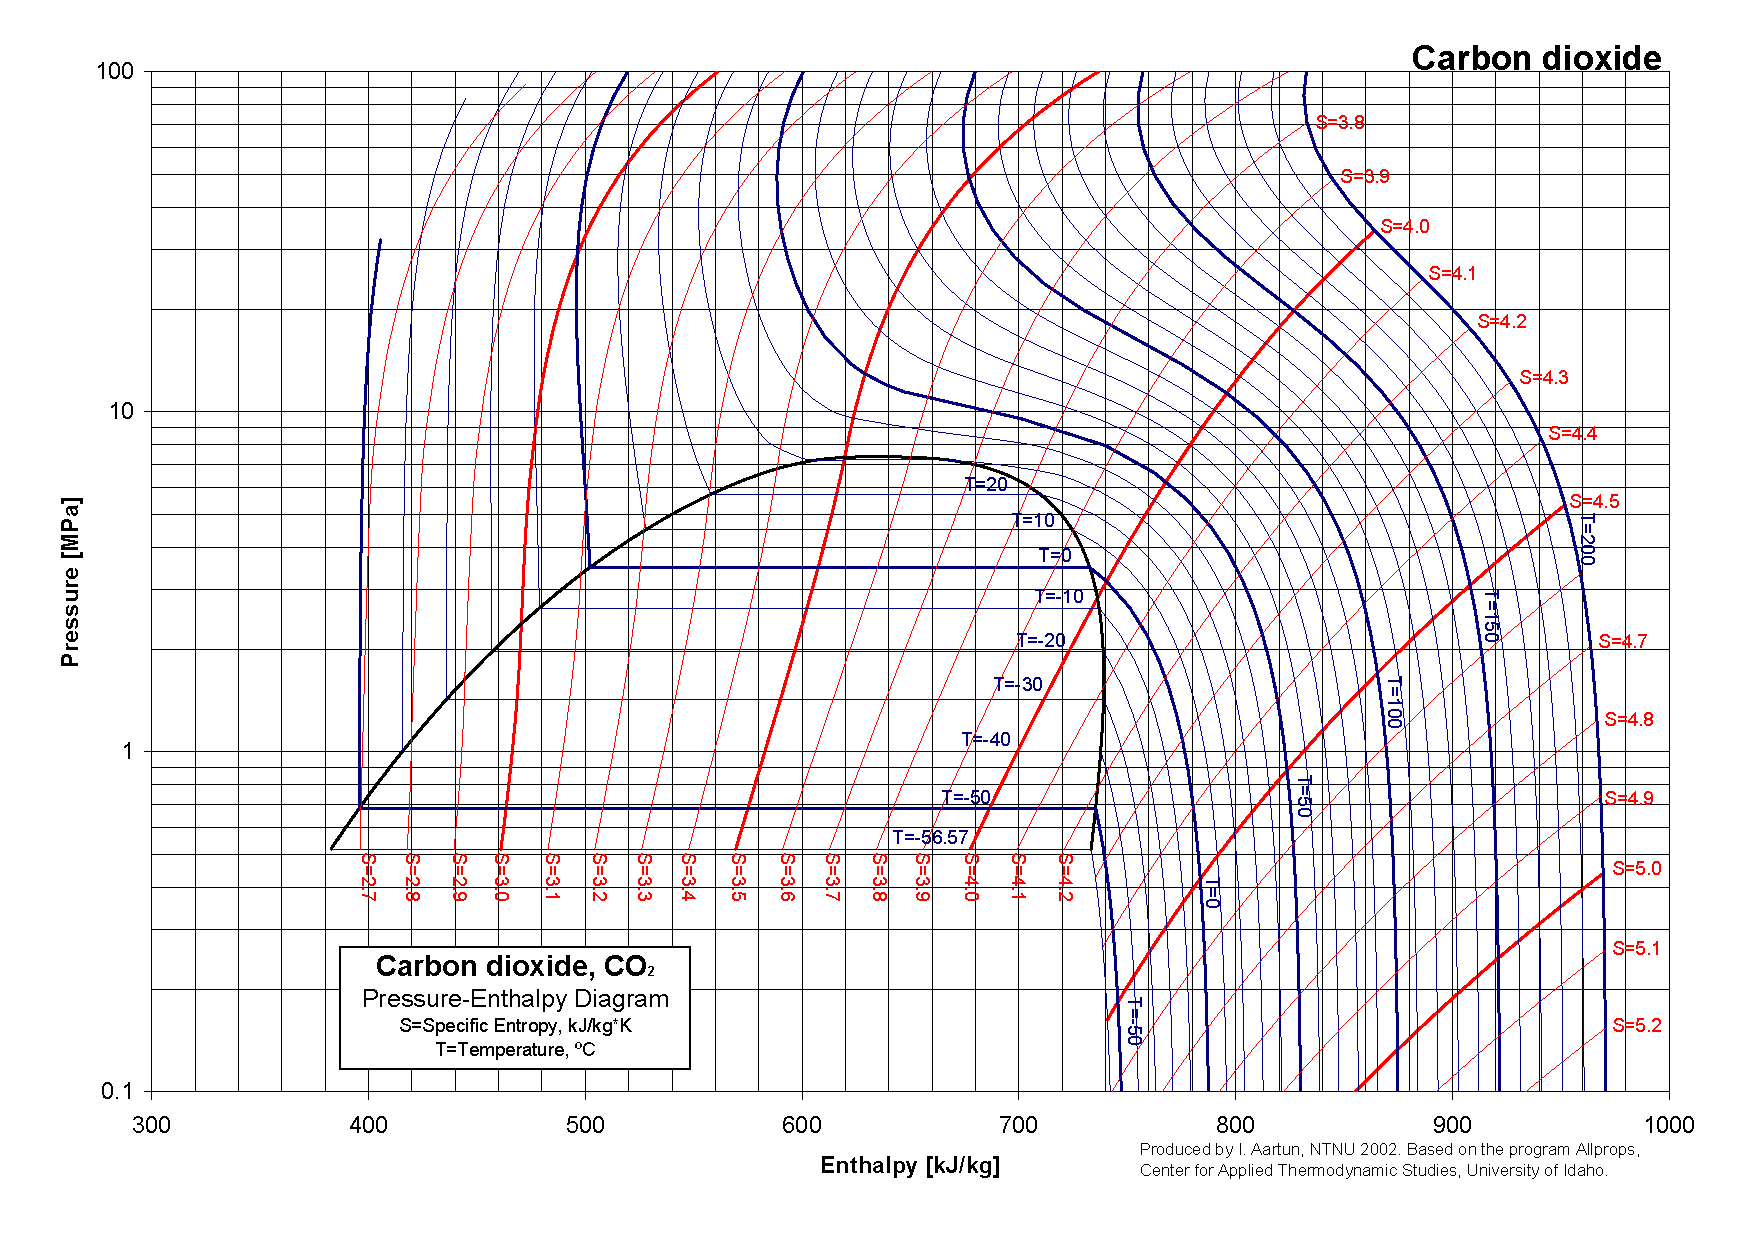
\includegraphics[width=9cm,height=8.cm,clip]{../Pics/CO2col}
   \end{figure}
   \end{center}
\end{frame}

%%%
%%% Slide
%%%
\begin{frame}
 \frametitle{Thermodynamics Diagrams: Pressure $\times$ Specific Enthalpy $(Ph)$}
  \begin{center}
   \begin{figure}
      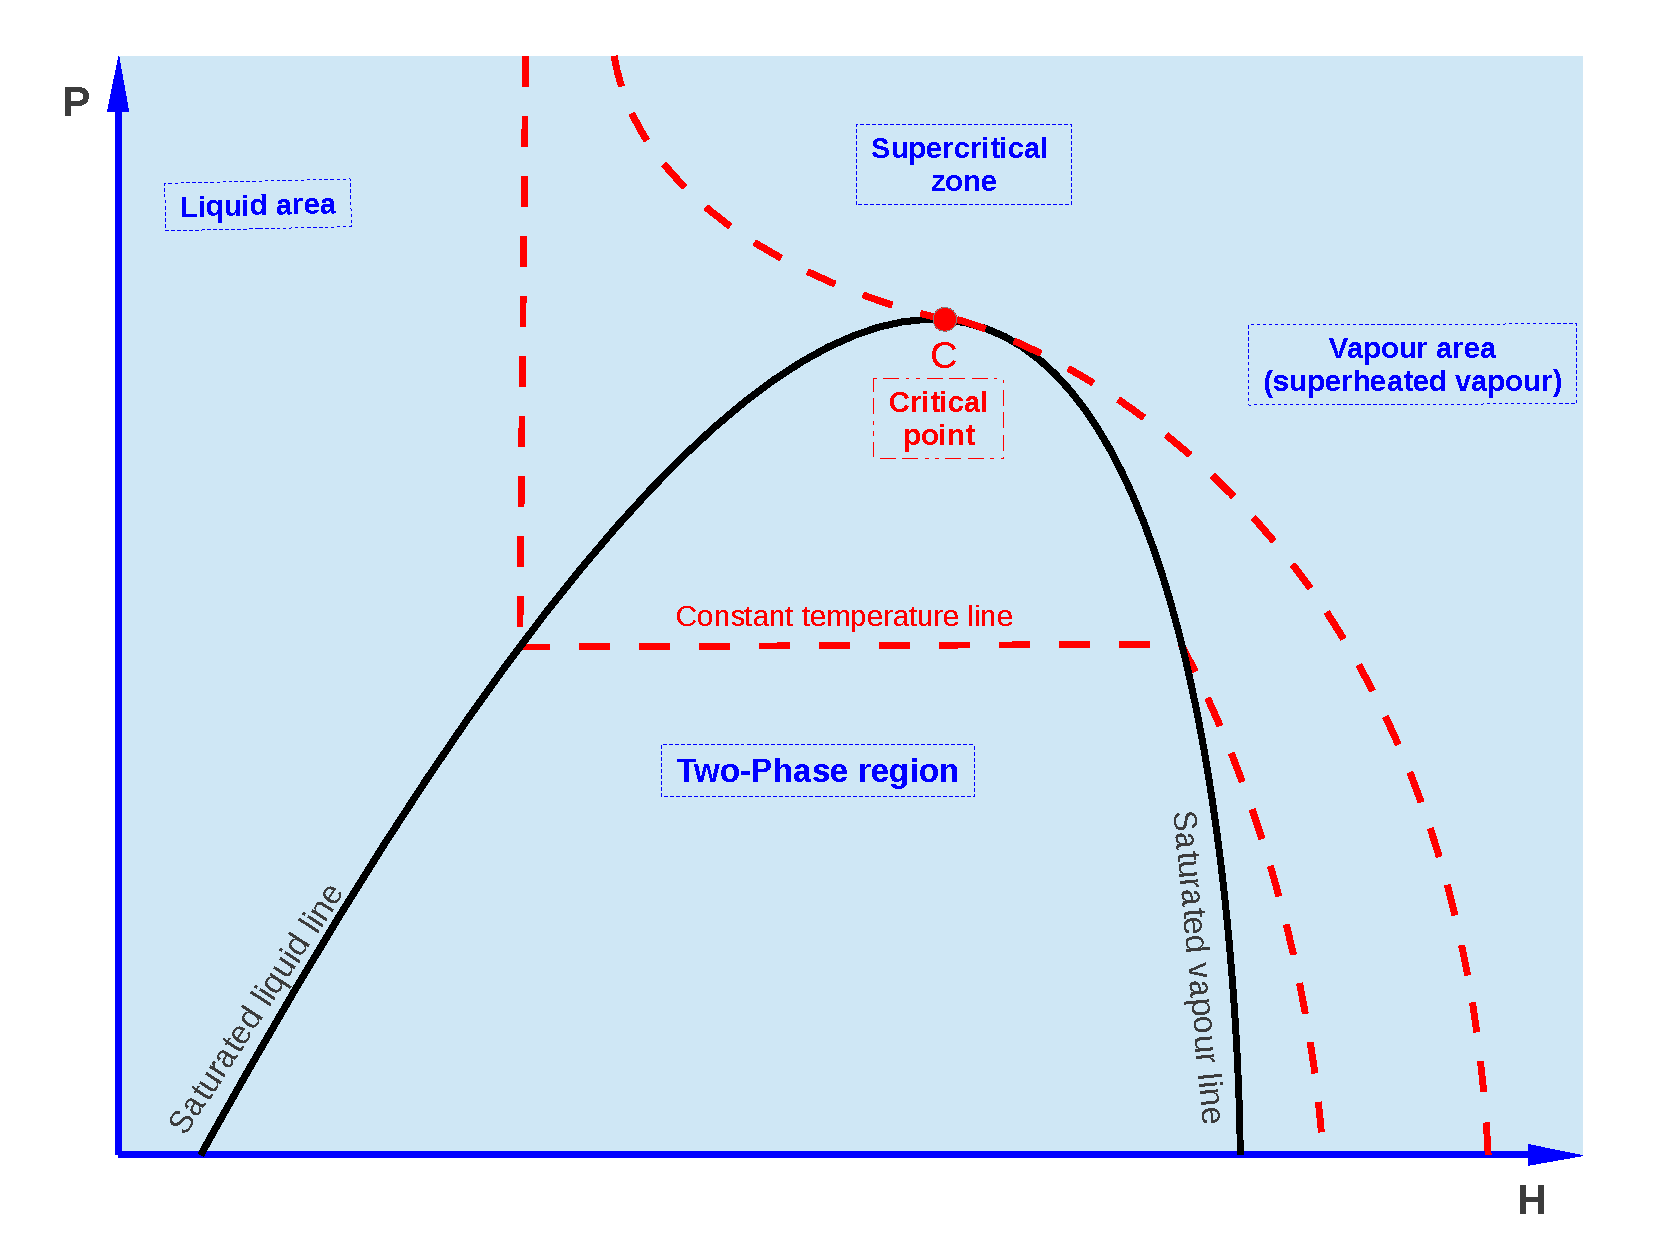
\includegraphics[width=8cm,height=7.cm,clip]{../Pics/Overview_Refrig18}
   \end{figure}
   \end{center}
\end{frame}

\begin{comment}
%%%
%%% Slide
%%%
\begin{frame}
 \frametitle{Thermodynamics Diagrams: Pressure $\times$ Specific Enthalpy $(Ph)$}
  \begin{center}
   \begin{figure}
      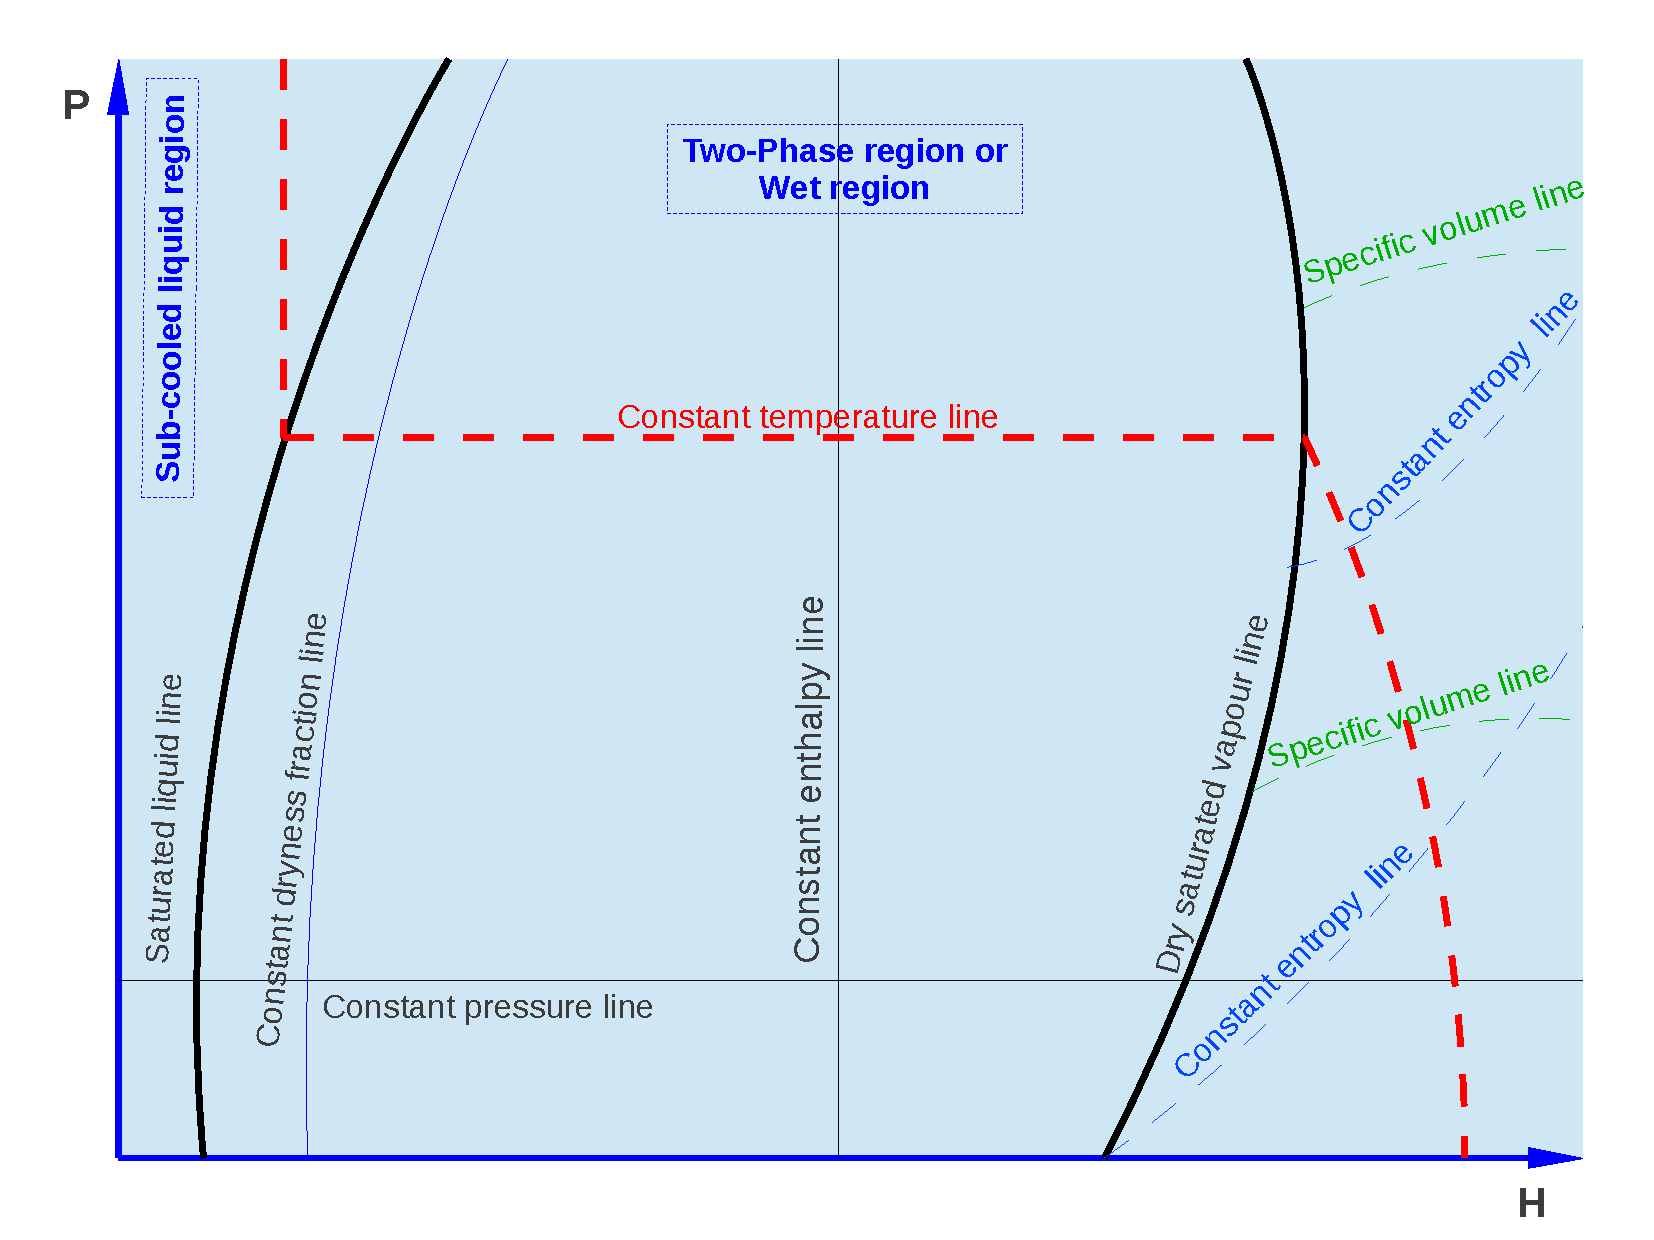
\includegraphics[width=8cm,height=7.cm,clip]{../Pics/Overview_Refrig17}
   \end{figure}
   \end{center}
\end{frame}
\end{comment}

%%%
%%% Slide
%%%
\begin{frame}
 \frametitle{Temperature $\times$ Specific Entropy $(Ts)$ Diagram for Water}
  \begin{center}
   \begin{figure}
     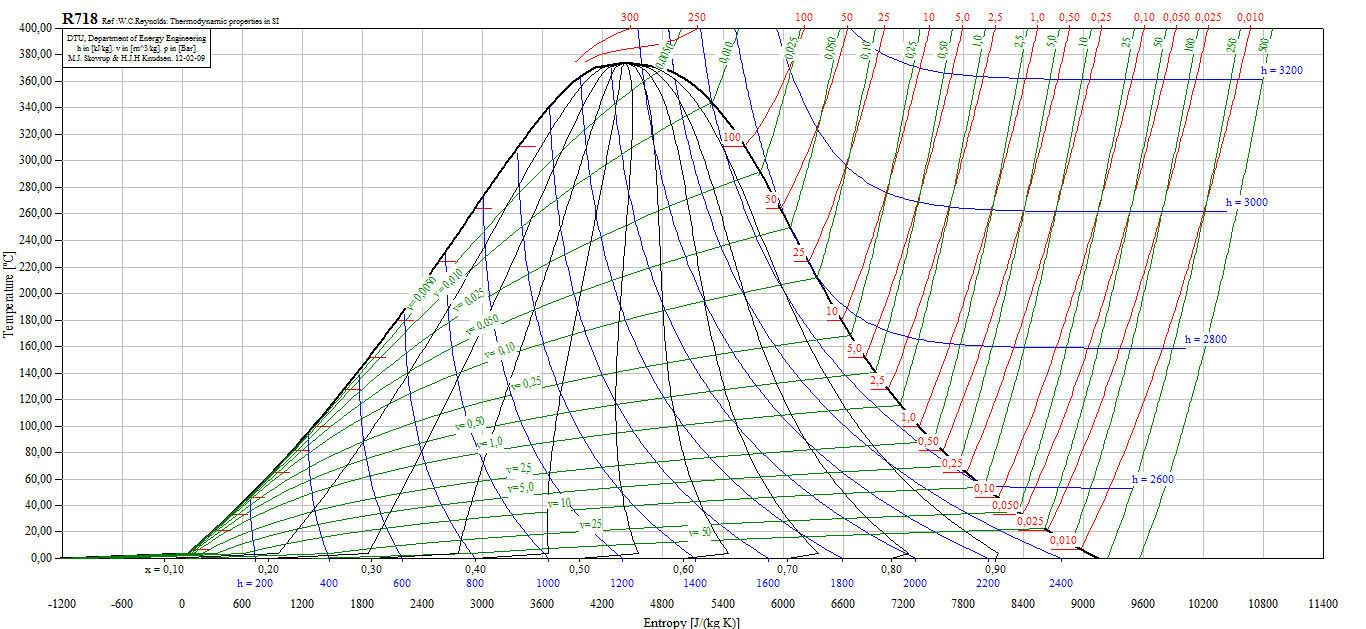
\includegraphics[width=8cm,height=7.cm,clip]{../Pics/water_TS.png}
   \end{figure}
   \end{center}
\end{frame}

%%%
%%% Slide
%%%
\begin{frame}
 \frametitle{Thermodynamics Diagrams: Temperature $\times$ Specific Entropy $(Ts)$}
  \begin{center}
   \begin{figure}
      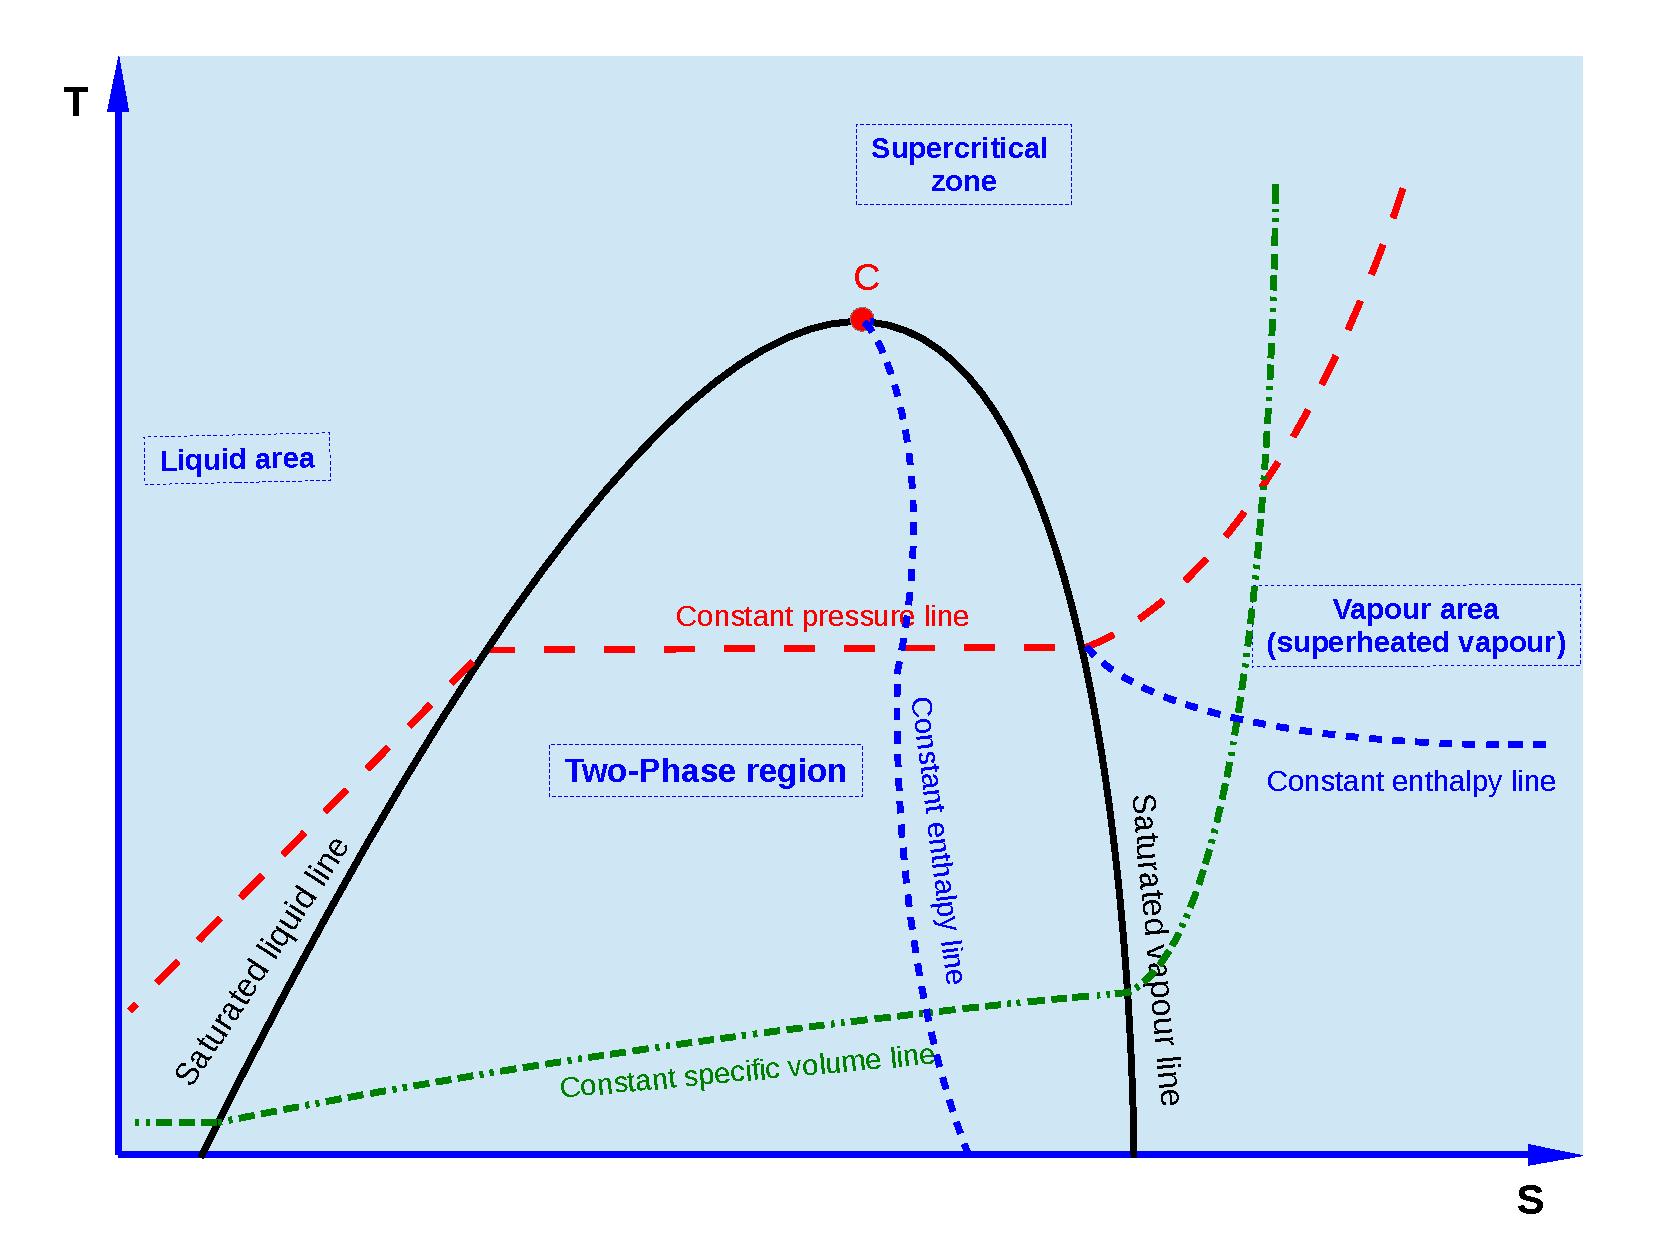
\includegraphics[width=8cm,height=7.cm,clip]{../Pics/TS_Diag_Schematics}
   \end{figure}
   \end{center}
\end{frame}

%%%
%%% Slide
%%%
\begin{frame}
  \frametitle{Another option: (a) \red{Saturated} and (b) Superheated Tables}
\scriptsize{From Reference [4]:}\vspace{-.8cm}
   \begin{center}
   \begin{figure}
      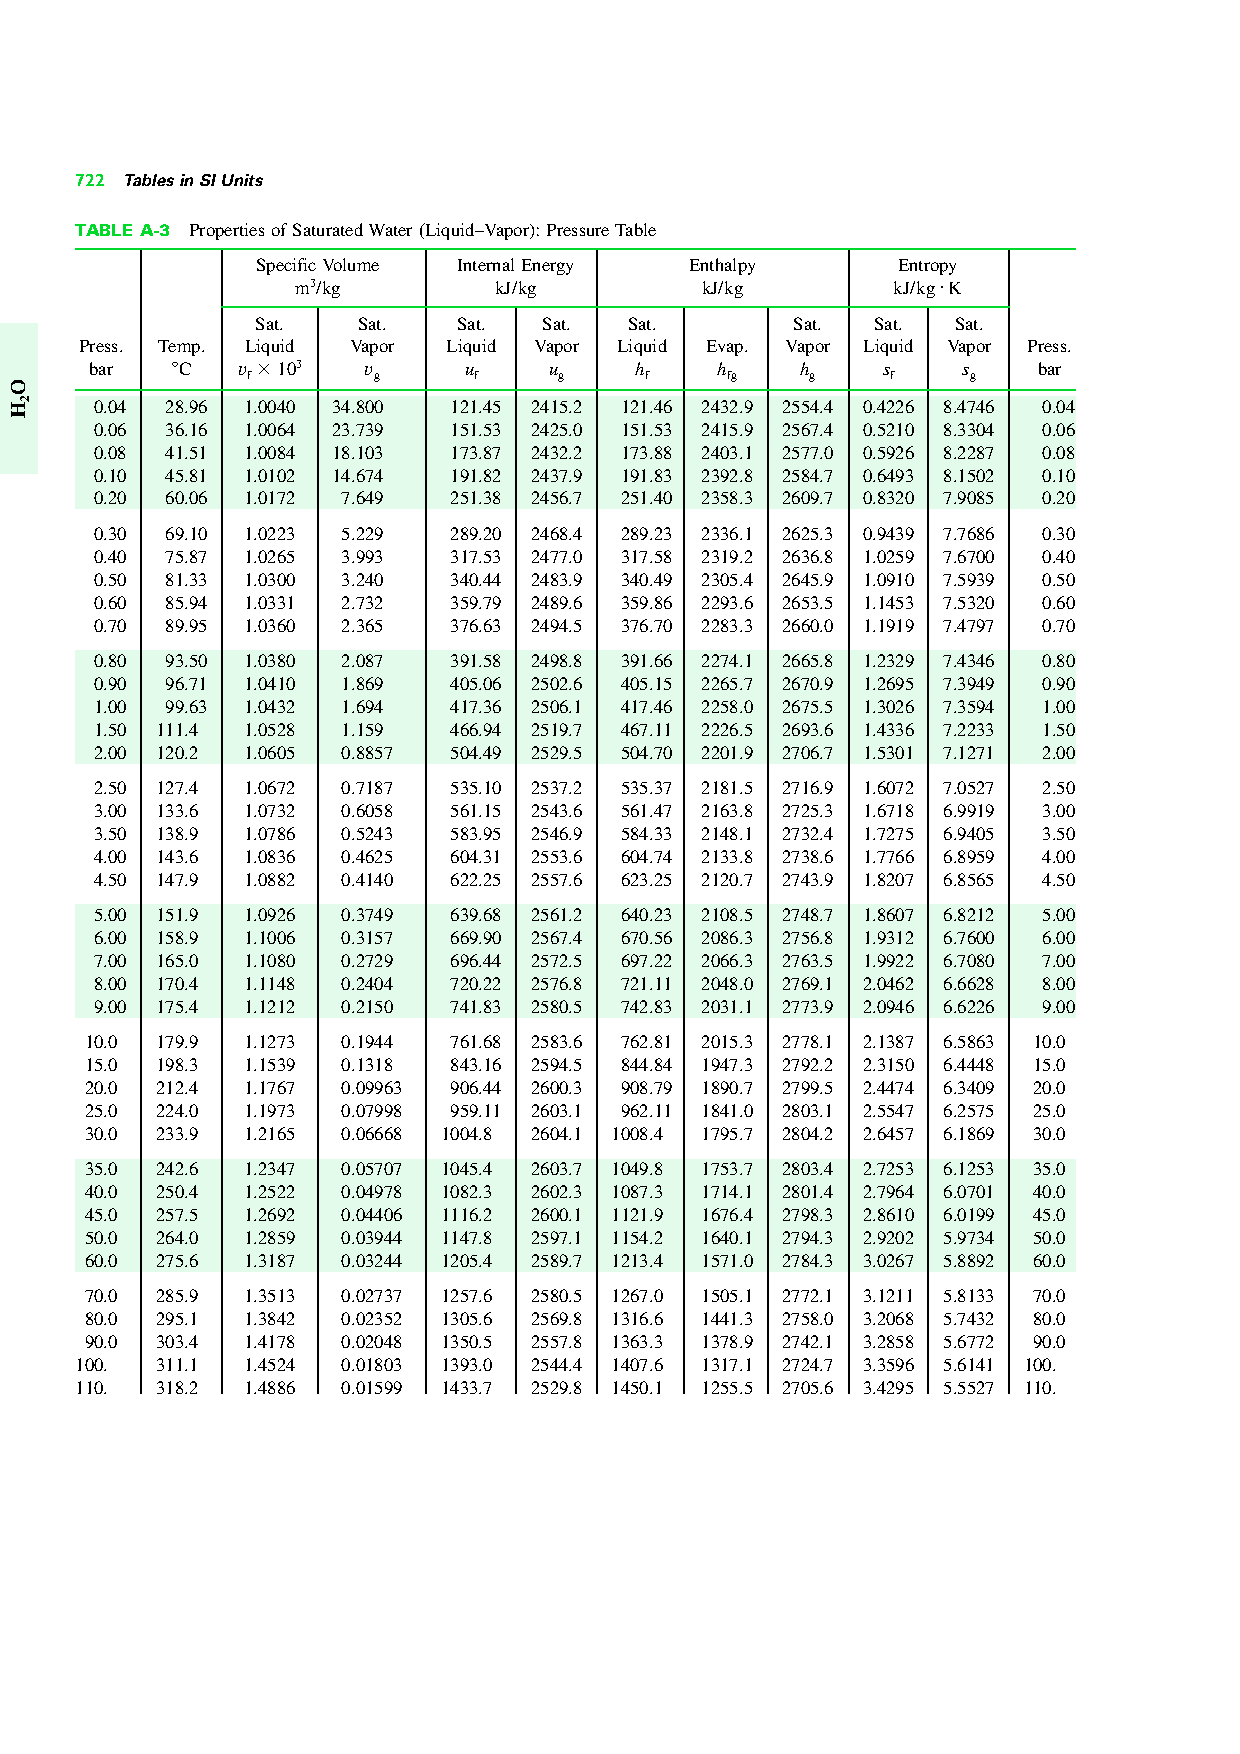
\includegraphics[width=9.cm,height=9.5cm,clip]{../Pics/WaterSatTable}
   \end{figure}
   \end{center}
\end{frame}

%%%
%%% Slide
%%%
\begin{frame}
  \frametitle{Another option: (a) Saturated and (b) \red{Superheated Tables}}
\scriptsize{From Reference (d):}\vspace{-.8cm}
   \begin{center}
   \begin{figure}
      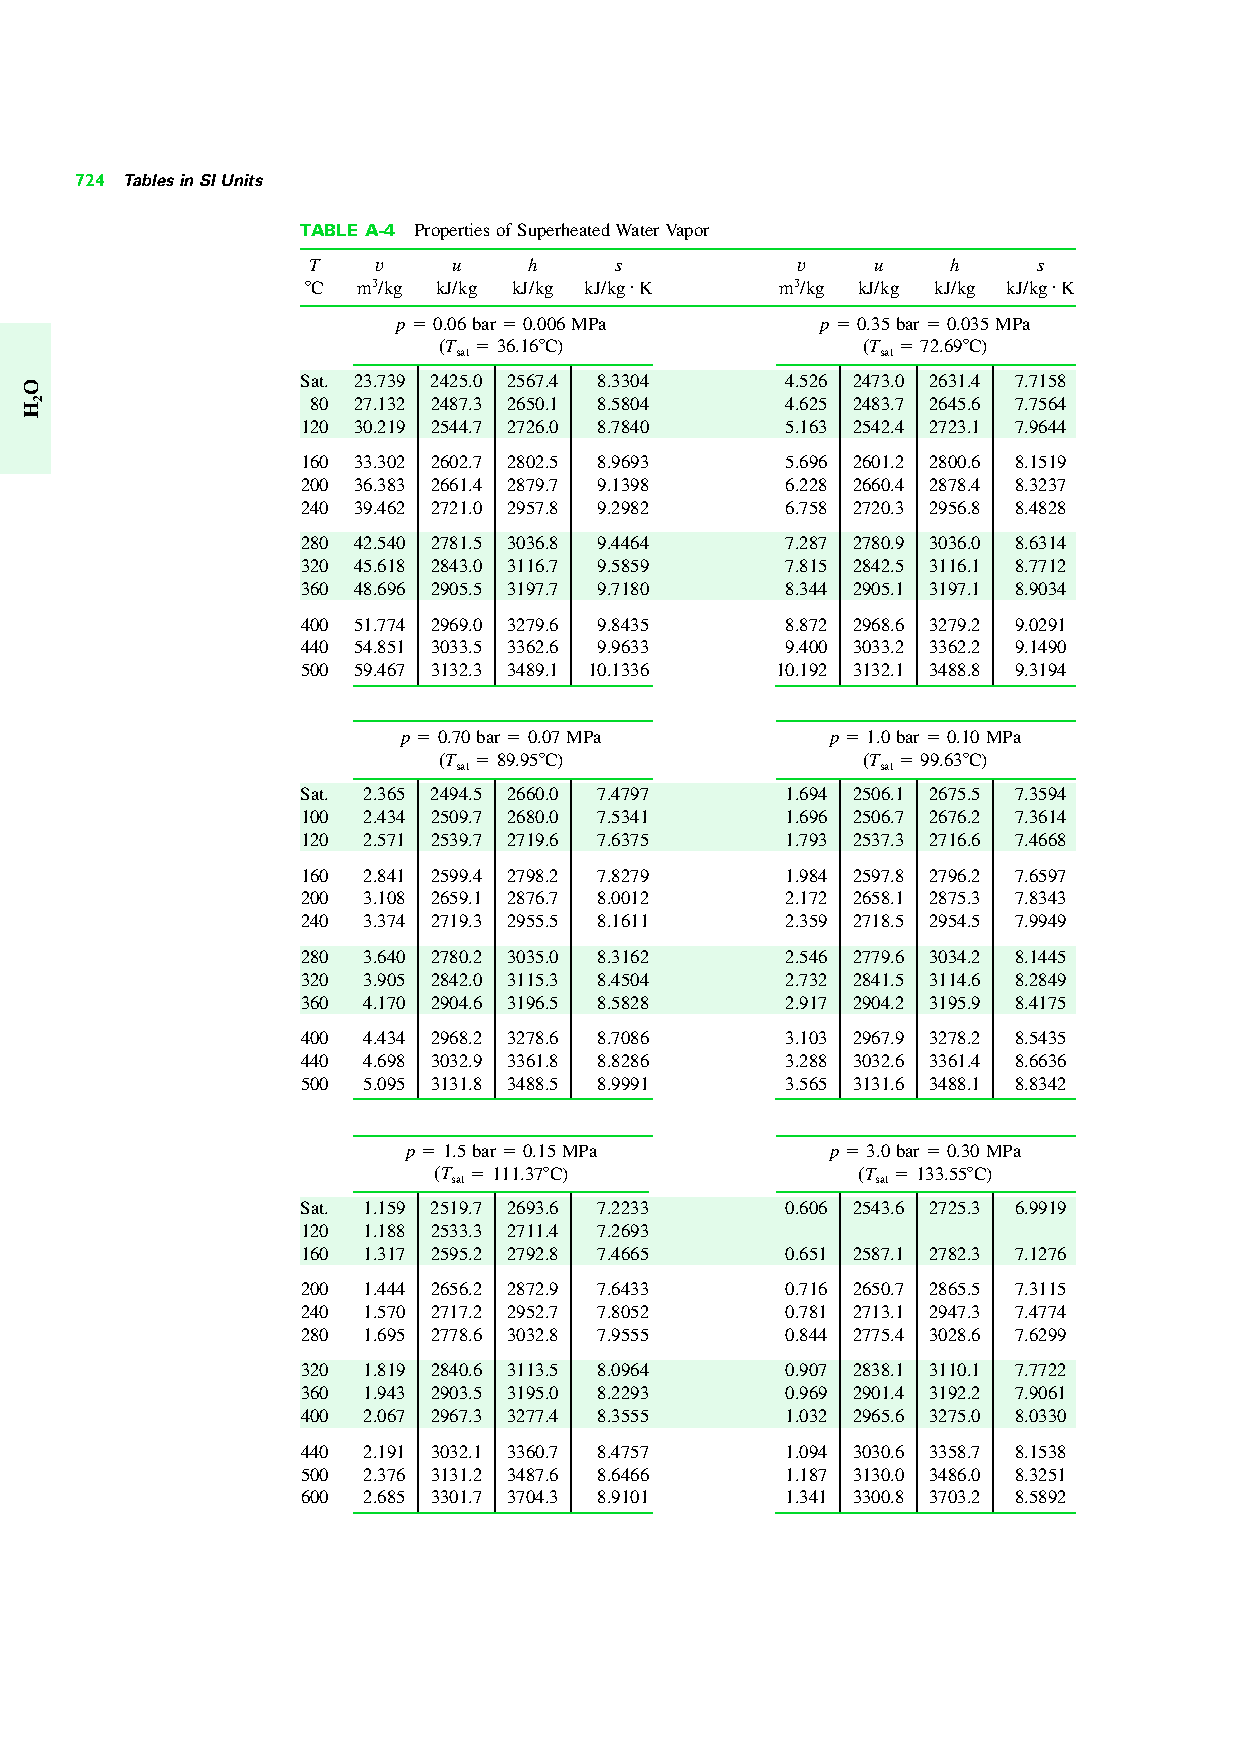
\includegraphics[width=9.5cm,height=8.5cm,clip]{../Pics/Water_SuperheatedTable} 
   \end{figure}
   \end{center}
\end{frame}

\begin{comment}
%%%
%%% Slide
%%%
\begin{frame}
  \frametitle{Another option: (a) Saturated and (b) Superheated Tables with (c) \red{Linear Interpolation}}
\noindent
\begin{enumerate}\scriptsize
\item <1-> {\bf \textcolor{red}{Example:}} At $P=1.50\;$ bar, the saturated steam has the following thermodynamic properties,
%\tiny 
\begin{center}
%\begin{table}[h]
\visible<2->{\begin{tabular}{c c|c c c|c c|c c} 
%\hline\hline
$P$ & $T$ & $h_{f}$ &  $h_{fg}$ & $h_{g}$ & $s_{f}$ &  $s_{g}$ & $v_{f}$ & $v_{g}$ \\ 
\hline
1.50 & 111.4 & 467.11 & 2226.5 & 2693.6 & 1.4336 & 7.2233 & 0.0010528 & 1.159 \\
%\hline
\end{tabular}
where: [$P$] = bar, [$T$] = $^{o}$C, [$h$]= $\frac{kJ}{kg}$, [$s$]=$\frac{kJ}{kg.K}$, [$v$]=$\frac{m^{3}}{kg}$.}
\end{center}

\item <3-> But the properties of superheated steam at the same pressure will depend on the temperature $\Rightarrow$ \textcolor{red}{see superheated steam table}. Thus at 1.50 bar $\left(\text{with }T_{\text{sat}}=111.4^{\circ}\text{C}\right)$:
  \visible<3->{\begin{center}\begin{tabular}{ c | c c c}
      $T$    & $v$    & $h$     &    $s$     \\
\hline
      111.4  & 1.159  & 2693.6  &  7.2233    \\
      120.0  & 1.188  & 2711.4  &  7.2693    \\
      160.0  & 1.317  & 2792.8  &  7.4665    \\
      200.0  & 1.444  & 2872.9  &  7.6433    \\
      240.0  & 1.570  & 2952.7  &  7.8052    \\ 
     $\vdots$& $\vdots$&$\vdots$&$\vdots$ \\
  \end{tabular}
  \end{center}
}
\item <4-> Some of the problems in this course involves extracting values from the thermodynamic tables;
\item <5-> And although the tables are very extensive (for most of the materials), sometimes we need values that can not be directly found on them;
\item <6-> In this case, we just operate a {\bf linear interpolation} between neighbour fields;
\item <7-> For example, \underline{water-steam at 1.50 bar and 212$^{o}$C};
\item <8-> At this pressure, the {\bf saturation temperature} is 111.3$^{o}$C, therefore we know that the fluid (water/steam) is at \textcolor{red}{superheated state};

\end{enumerate}

\end{frame}

%%%
%%% Slide
%%%
\begin{frame}
  \frametitle{Another option: (a) Saturated and (b) Superheated Tables with (c) \red{Linear Interpolation}}
\noindent
\begin{enumerate}\setcounter{enumi}{7}\scriptsize
\item <1-> Thus at 1.50 bar and 212$^{\circ}$C, enthalpy and entropy of superheated steam are within the following interval:
  \visible<1->{\begin{center}\begin{tabular}{ c | c c c}
      $T$    & $v$    & $h$     &    $s$     \\
      \textcolor{red}{200.0}  & 1.444  & \textcolor{red}{2872.9}  &  7.6433    \\
      \textcolor{red}{240.0}  & 1.570  & \textcolor{red}{2952.7}  &  7.8052    \\ 
  \end{tabular}
  \end{center}
}
\item<2-> The enthalpy at 212$^{o}$C can be calculated as,
\visible<3->{\begin{tabular}{ l l }
\scriptsize $\Delta T=T_{2}-T_{1}=240-200^{o}$C   & \scriptsize $\longleftrightarrow$  $\Delta h=h_{2}-h_{1}=2952.7-2872.9=79.8\frac{kJ}{kg}$ \\
\scriptsize $\Delta T^{\star} = T_{2} - T^{\star}= 240 - 212^{\circ}$C & \scriptsize $\longleftrightarrow$  $\Delta h^{\star}= h_{2} - h^{\star}= 2952.7 - h^{\star}$\\    
\end{tabular}}
\item <4-> $\Delta h^{\star}=55.86\frac{kJ}{kg}$ 
\item <4-> Thus $\Delta h^{\star}= h_{2}-h^{\star} \longrightarrow h\left(T=212^{\circ}C\right)=h^{\star}=2896.84\frac{kJ}{kg}$.
\item<5-> Similarly for entropy: $s\left(T=212^{\circ}C\right)=s^{\star}=7.6919\frac{kJ}{kg.K}$.
\end{enumerate}

\end{frame}

\end{comment}

%%%
%%% Slide
%%%

\begin{frame}
  \frametitle{Third Option: PVT Software and Websites}
\noindent
\begin{enumerate}[i)]
   \item<1-> \href{http://www.weatherford.com/doc/wft183650}{PVTflex$^{TM}$};
   \item<1-> \href{http://www.kbcat.com/infochem-software/flow-assurance-software-multiflash/pvt-simulation}{Multiflash$^{TM}$};
   \item<1-> \href{http://home.aspentech.com/products/engineering/aspen-hysys}{Aspen HYSIS};
   \item<1-> \href{https://www.honeywellprocess.com/en-US/explore/products/advanced-applications/unisim/Pages/default.aspx}{UniSim – Software for Process Design and Simulation};
   \item<1-> \href{http://webbook.nist.gov/chemistry/fluid/}{NIST Website}
   \item<1-> etc.
\end{enumerate}

\end{frame}


\subsection{Phase Transition}
%%%
%%% Slide
%%%
%\scriptsize
\begin{frame}
  \frametitle{General Remarks}
     \begin{enumerate}[i)]
         \item<1-> \textcolor{blue}{Phase transition}: many extensive properties change abruptly during phase transition at given $P$ and $T$: specific volume, internal energy, enthalpy and entropy;
         \item<2-> \textcolor{blue}{Exception:} \textcolor{red}{molar Gibbs energy};
         \item<3-> For an arbitrary number of phases $\left(\mathcal{P}=\left\{\alpha, \beta, \gamma, \cdots\right\}\right)$ of pure species $\left(\mathcal{C}=1\right)$ at equilibrium,
            \visible<3->{\begin{block}{\begin{center}\blue{\normalsize{Equilibrium $\Rightarrow$ Equality of Gibbs energy}}\end{center}}
                     \begin{displaymath}
                        \red{G^{\alpha} = G^{\beta} = G^{\gamma} = \cdots } 
                     \end{displaymath}
            \end{block}}
         \item<4-> When a pure component is in equilibrium, \red{\it all coexisting phases have the same temperature and pressure};
     \end{enumerate}

\end{frame}
\normalsize

%%%
%%% Slide
%%%
%\scriptsize
\begin{frame}
  \frametitle{Clapeyron Relations}
     \begin{enumerate}[i)]\setcounter{enumi}{4}
         \item<1-> Let's consider a pure substance where phases $\alpha$ and $\beta$ are in thermodynamic equilibrium (\ie two-phase system). The Gibbs free energy for both phases can be expressed as
              \visible<1->{\begin{displaymath}
                              V^{\alpha} dP^{\text{sat}} - S^{\alpha}dT = V^{\beta} dP^{\text{sat}} - S^{\beta}dT,
                           \end{displaymath}
              where $P^{\text{sat}}$ is the saturated pressure, \ie pressure in which phase change occurs.}
         \item<2-> This expression can be manipulated to obtain 
                 \visible<2->{\begin{block}{\begin{center}\normalsize{Clapeyron Equation}\end{center}}
                                  \begin{displaymath}
                                      \frc{dP^{\text{sat}}}{dT} = \frc{\Delta H^{\alpha\beta}}{T\Delta V^{\alpha\beta}},
                                  \end{displaymath}
                  where $\Delta H^{\alpha\beta}$ is the {\it latent heat of phase transition} (\eg vaporisation, solidification etc). 
                  \end{block}
   }
        
     \end{enumerate}

\end{frame}
\normalsize

%%%
%%% Slide
%%%
%\scriptsize
\begin{frame}
  \frametitle{Clapeyron Relations}
     \begin{enumerate}[i)]\setcounter{enumi}{6}
         \item<1-> For liquid-vapour phase changes and assuming that the vapour phase behaves as an ideal gas, 
             \visible<1->{\begin{displaymath}
                            \frc{dP^{\text{sat}}}{dT} = \frc{P^{\text{sat}}\Delta H^{\text{fg}}}{RT^{2}},
                          \end{displaymath}}
         \item<2-> And assuming that at {\it infinitesimal intervals of } $T$, $\Delta H^{\text{fg}}$ can be considered as constant,
             \visible<2->{\begin{displaymath} 
                            \frc{d\left(\ln{P^{\text{sat}}}\right)}{dT} = \frc{\Delta H^{\text{fg}}}{RT^{2}} \;\;\Longrightarrow \;\;\; \ln{\left(\frc{P_{2}}{P_{1}}\right)_{\text{sat}}} = \frc{\Delta H^{\text{fg}}}{R}\left(\frc{1}{T_{1}}-\frc{1}{T_{2}}\right)_{\text{sat}}
                          \end{displaymath}}
     \end{enumerate}

\end{frame}
\normalsize


%%%
%%% Slide
%%%
%\scriptsize
\begin{frame}
  \frametitle{Clapeyron Relations}
     \begin{enumerate}[i)]\setcounter{enumi}{8}
         \item<1-> The temperature dependence of saturation pressure led to number of empirical expressions for practical applications, \eg
         \begin{enumerate}[a)]
            \item<2-> Simplest case:
                \visible<2->{\begin{displaymath}
                   \ln P^{sat} = A - \frc{B}{T}
                \end{displaymath}}
            \item<3-> Antoine Equation:
                \visible<3->{\begin{displaymath}
                   \ln P^{sat} = A - \frc{B}{T+C}
                \end{displaymath}}
            \item<4-> Wagner Equation \blue{(more accurate)}:
                \visible<4->{\begin{displaymath}
                   \ln P_{r}^{sat} = \frc{A\tau + B\tau^{1.5} + C\tau^{3} + D\tau^{6}}{1-\tau}\;\;\;\text{ with }\;\;\; \tau = 1 - T_{r}
                \end{displaymath}}
         \end{enumerate}
     \end{enumerate}

\end{frame}
\normalsize


%%%
%%% SUBSECTION 
%%%
\subsection{Liquid/Vapour Systems}
%%%
%%% Slide
%%%
%\scriptsize
\begin{frame}
  \frametitle{Liquid/Vapour Systems}
     \begin{enumerate}[(a)]
         \item<1-> Systems with \blue{saturated vapour} and \blue{saturated liquid} in \red{equilibrium};
         \item<2-> \blue{Mass/Energy Balance} for any extensive property:
            \visible<3->{\begin{displaymath} 
                nV = n^{(l)}V^{(l)} + n^{(v)}V^{(v)} \;\;\; \Leftrightarrow \;\;\; V = x^{(l)}V^{(l)} + x^{(v)}V^{(v)}
             \end{displaymath}
             where $x^{(j)}$ is the \blue{molar/mass fraction} of phase \blue{j = l, v} $\rightarrow$  $x^{(l)} + x^{(v)} = 1$. 
            }
         \item<4-> The mass/molar volume fraction of vapour, \blue{$x^{(v)}$}, is also called \blue{vapour quality}. 
     \end{enumerate}

\end{frame}
\normalsize

%%%
%%% Slide
%%%
\begin{frame}
 \frametitle{Applications of Liquid-Vapour System: Steam Power Plants}
 %\scriptsize

    \begin{enumerate}%\scriptsize
     \item <1-> While coal, natural gas, and nuclear still play important roles as energy sources, contributions from wind power, solar power, and other renewable sources are expected to be increasingly significant up to 2050;
     \item <3-> The basic building block of vapour power systems is the \blue{Rankine cycle};
     \item <4-> Energy sources based on thermal-cycles (YouTube videos):
        \begin{itemize}%\scriptsize
           \item \href{http://www.youtube.com/watch?v=_UwexvaCMWA}{\textcolor{blue}{Nuclear Power Plants (NPP)}};
           \item \href{http://www.youtube.com/watch?v=0mjT8ETB128}{\textcolor{blue}{Coal-Fired Stations}};
           \item \href{http://www.youtube.com/watch?v=oi1TRbiE_Kw}{\textcolor{blue}{Gas Turbine Combined Cycle Power Plant}};
           \item \href{https://www.youtube.com/watch?v=kjpp2MQffnw}{\textcolor{blue}{Geothermal Power Plant}}.
        \end{itemize}
    \end{enumerate} 
 \normalsize
\end{frame}


%%%
%%% Slide
%%%
\begin{frame}
 \frametitle{Rankine Cycle}
 %\scriptsize
 \begin{columns}
   \begin{column}[c]{0.5\linewidth}
    \begin{figure}%
     \begin{center} 
      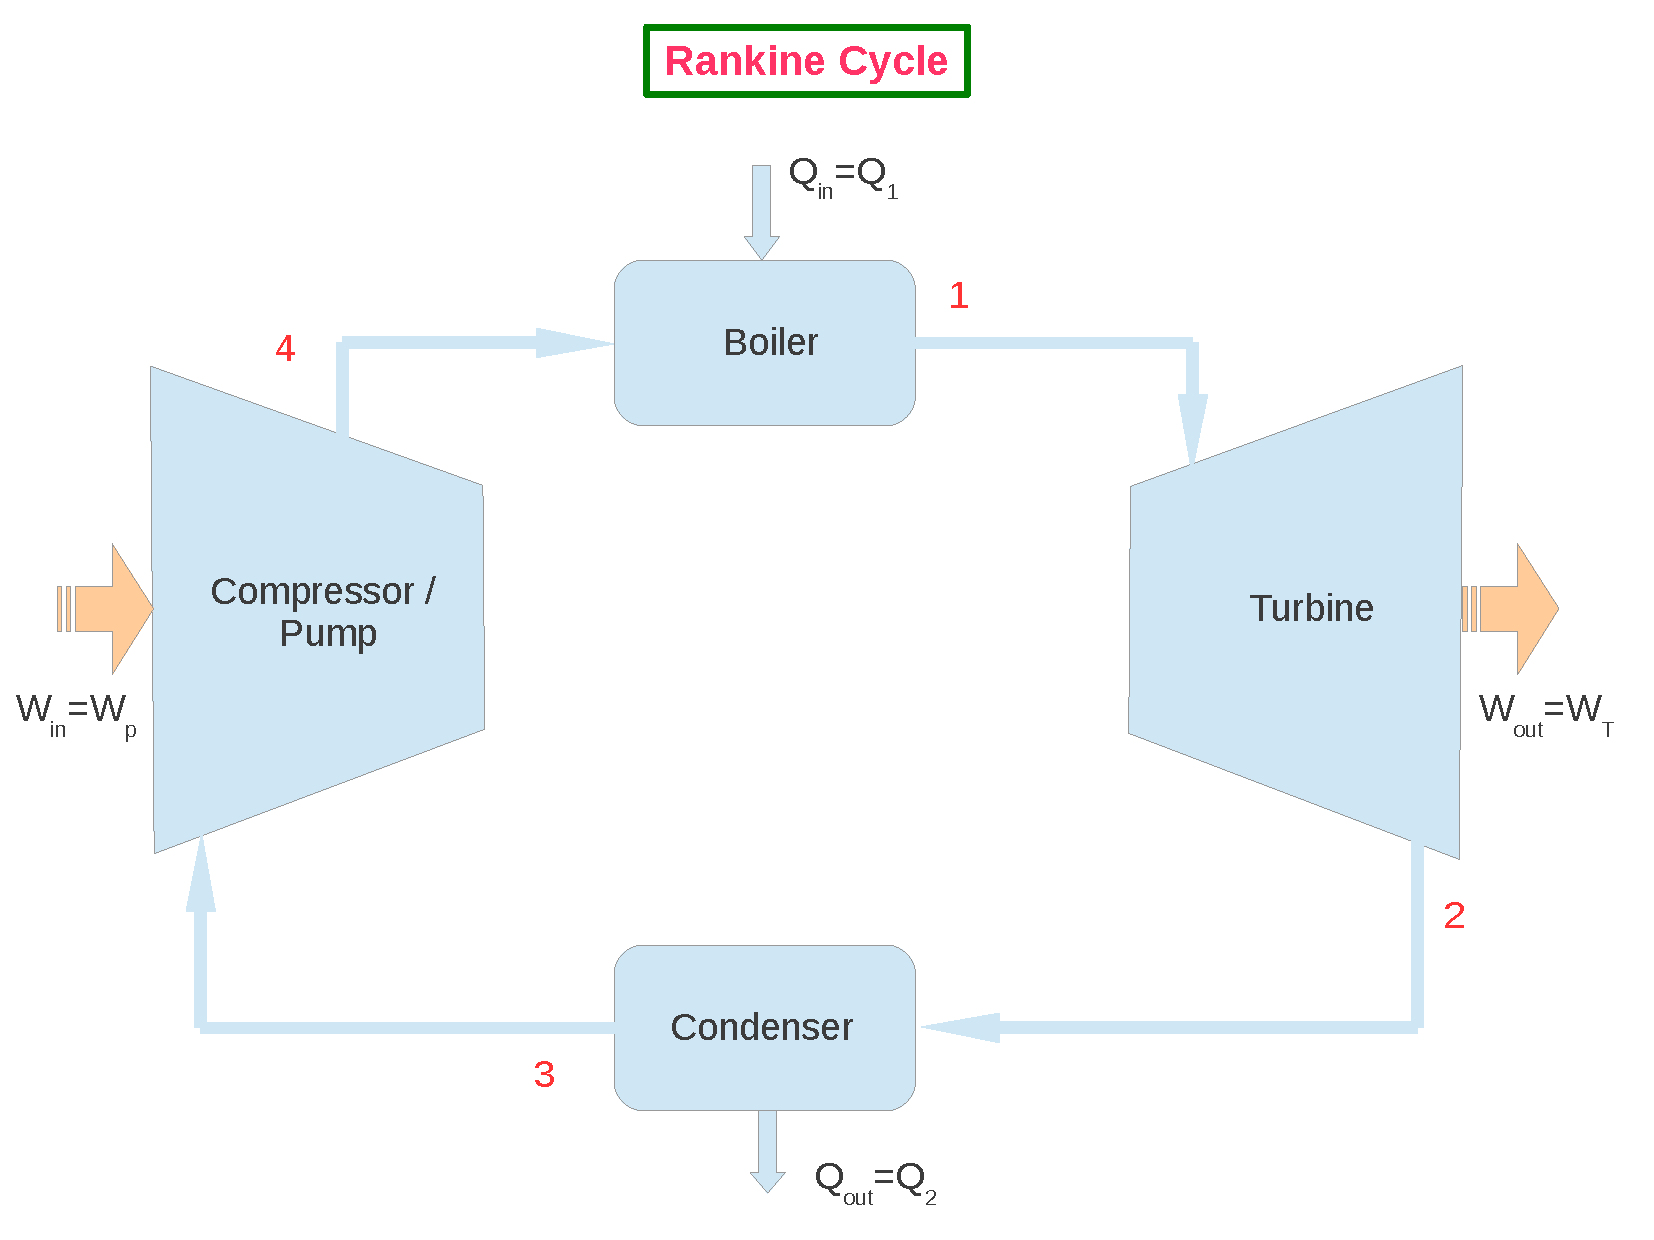
\includegraphics[width=6.5cm,clip]{../Pics/Simple_Rankine_Cycle}
     \end{center}
    \end{figure}  
   \end{column}
   \begin{column}[l]{0.5\linewidth}
    \begin{enumerate}[i)]\scriptsize
     \item<1->\blue{Rankine Cycle} (RC) is the ideal cycle for vapour power plants;
     \item<2-> It does not involve any internal irreversibilities and consists of the following four processes:
     \begin{enumerate}[a)]\scriptsize
      \item<3-> \red{Process 1-2}: reversible adiabatic (i.e., \blue{isentropic}) expansion in the turbine (or steam engine);
      \item<4-> \red{Process 2-3}: constant-pressure heat transfer in the condenser;
      \item<5-> \red{Process 3-4}: reversible adiabatic (i.e., \blue{isentropic}) pumping process in the feed pump;
      \item<6-> \red{Process 4-1}: constant-pressure heat transfer in the boiler.  
     \end{enumerate}
     \item<7-> Efficiency of the \blue{RC} can be expressed as:
       \visible<7->{\begin{eqnarray}
          \blue{\eta_{\text{Rankine}}} &=& \frc{W_{\text{net}}}{Q_{1}} = \frc{W_{T}-W_{P}}{Q_{1}}\nonumber \\
                                    &=& \frc{\left(h_{1}-h_{2}\right)-\left(h_{f4}-h_{f3}\right)}{h_{1}-h_{f4}} \nonumber \\
                                    &=& \blue{\frc{h_{1}-h_{2}}{h_{1}-h_{f4}}}  \nonumber
       \end{eqnarray}}
    \end{enumerate}
   \end{column}
  \end{columns}
 \normalsize
\end{frame}


%%%
%%% Slide
%%%
\begin{frame}
 \frametitle{Rankine Cycle: {\it Pv}, {\it Ts} and {\it hs} Diagrams}
 %\scriptsize
 \begin{columns}
%
   \begin{column}[l]{0.45\linewidth}
    \begin{figure}%
     \begin{center}
      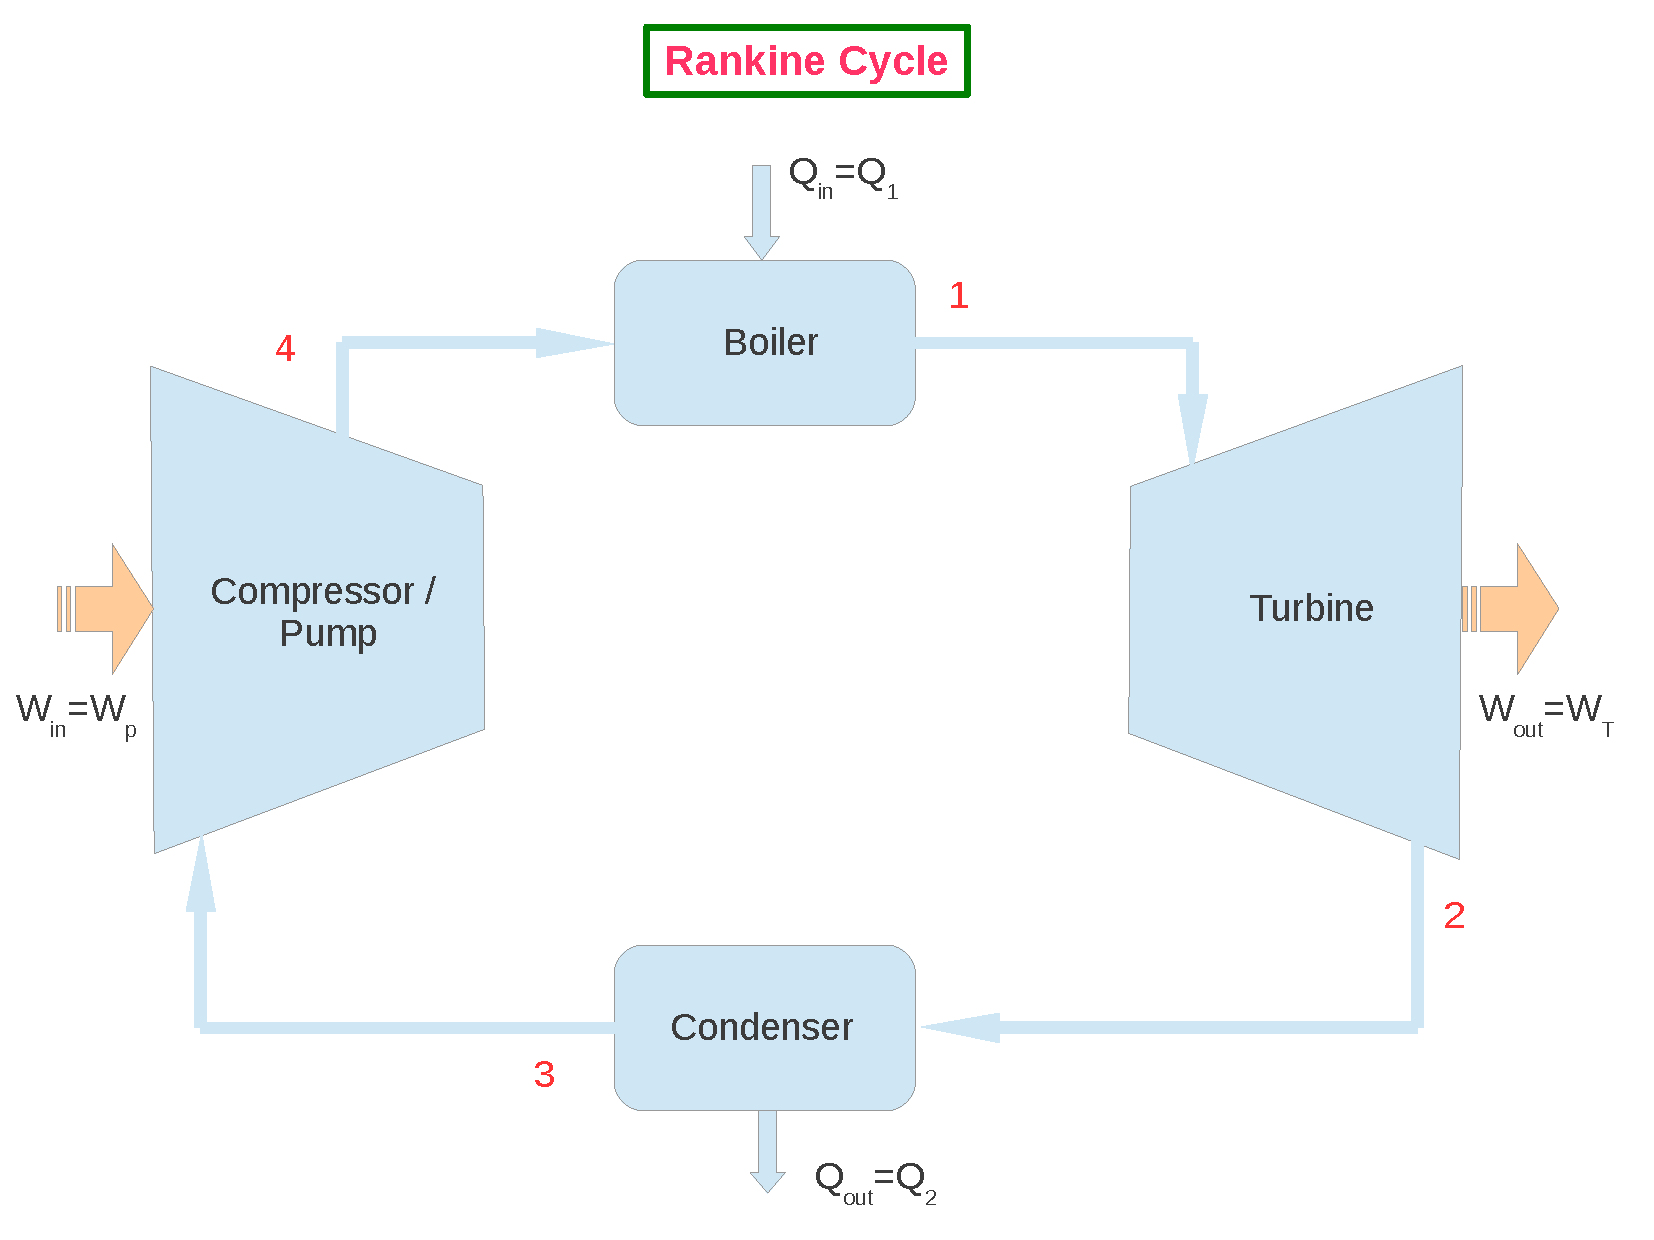
\includegraphics[width=5.5cm,clip]{../Pics/Simple_Rankine_Cycle}
     \end{center}
    \end{figure} 
    \begin{block}{\begin{center}Quality of the Vapour\end{center}}
       \begin{displaymath}\scriptsize
         \blue{x_{j} = \frc{\Psi_{j}-\Psi_{f}}{\Psi_{g}-\Psi_{f}}} \;\;\;\text{with }\Psi=\left\{h,s\right\}
       \end{displaymath}
    \end{block}
   \end{column}
%
   \begin{column}[c]{0.55\linewidth}
    \begin{figure}%
     \begin{center}
      \visible<2->{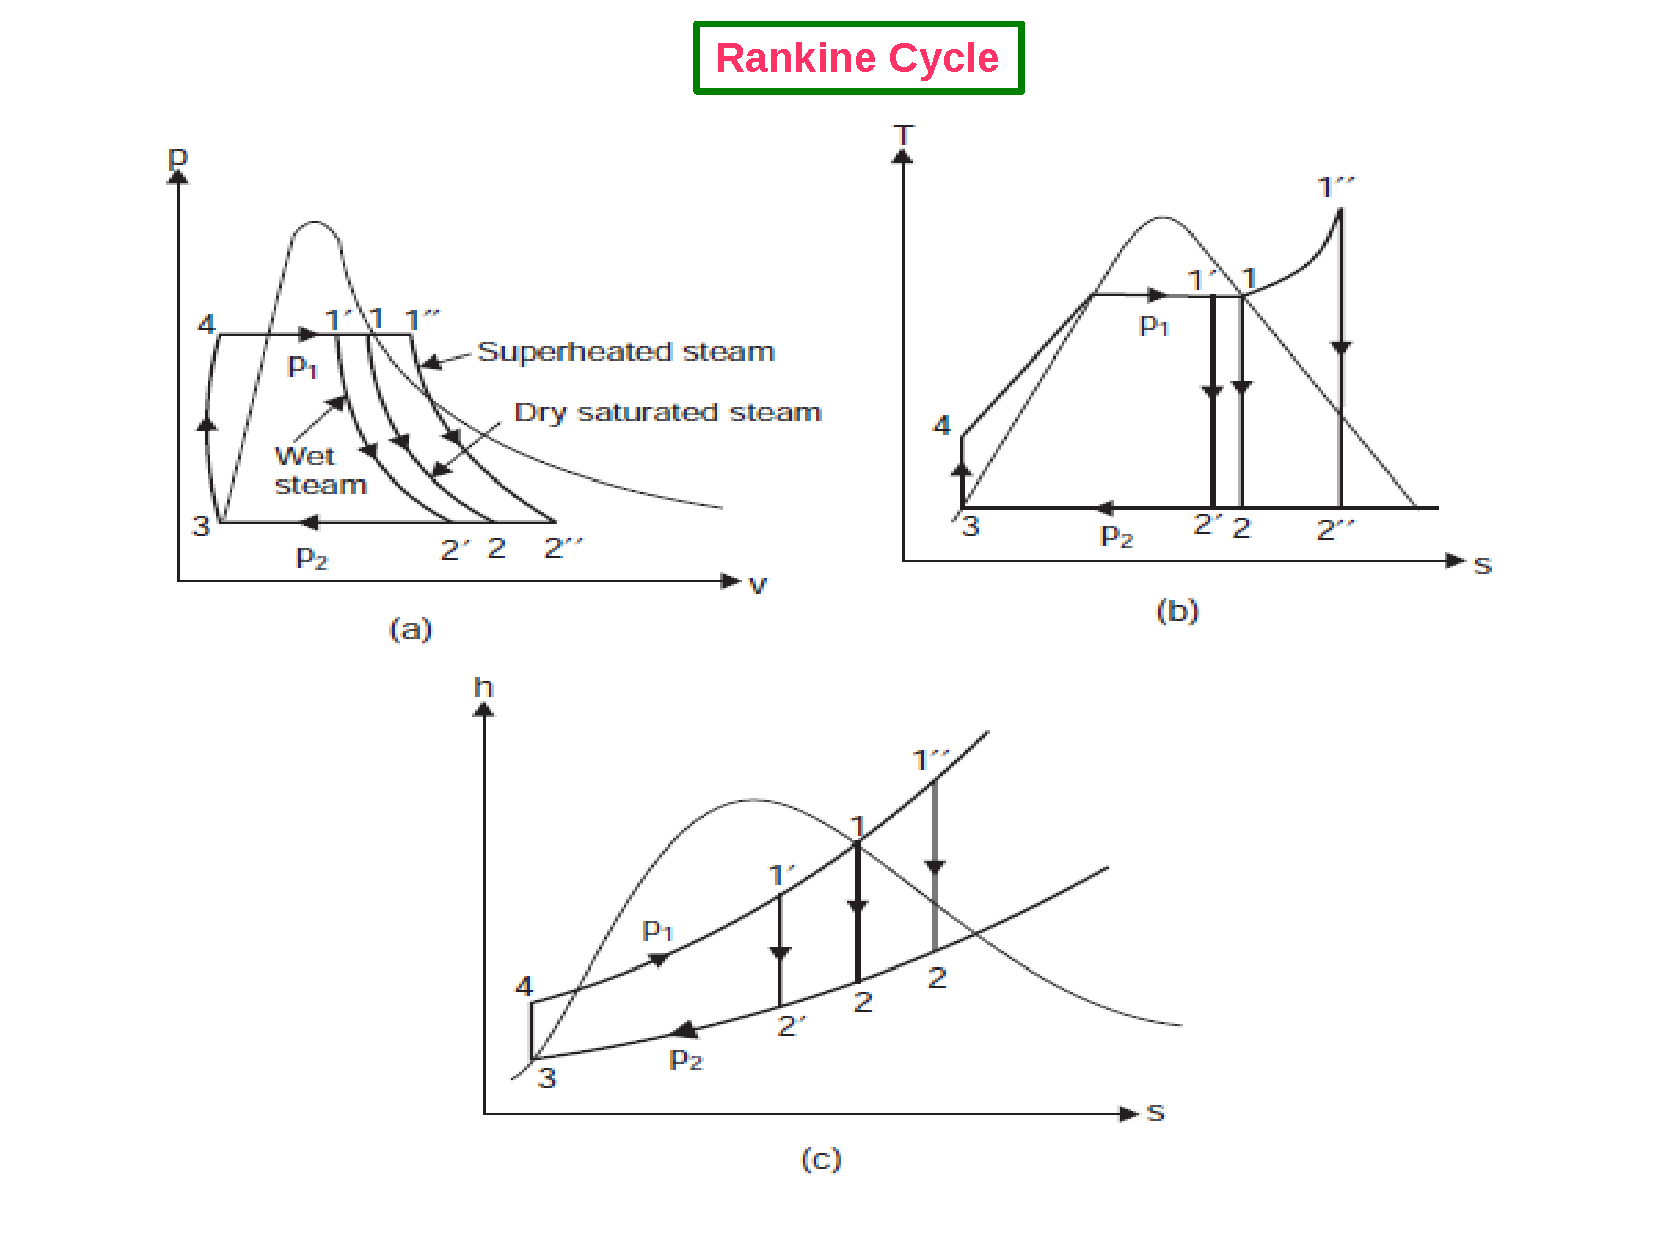
\includegraphics[width=7.5cm,clip]{../Pics/Simple_Rankine_Cycle_Diagrams}}
     \end{center}
    \end{figure}  
   \end{column}
  \end{columns}
\end{frame}


%%%
%%%  COMMENT
%%%
\begin{comment}
%%%
%%% Slide
%%%
%\scriptsize
\begin{frame}
  \frametitle{Pressure $\times$ Enthalpy ({\it PH}) Diagram}
      \begin{figure}%
        \begin{center}
          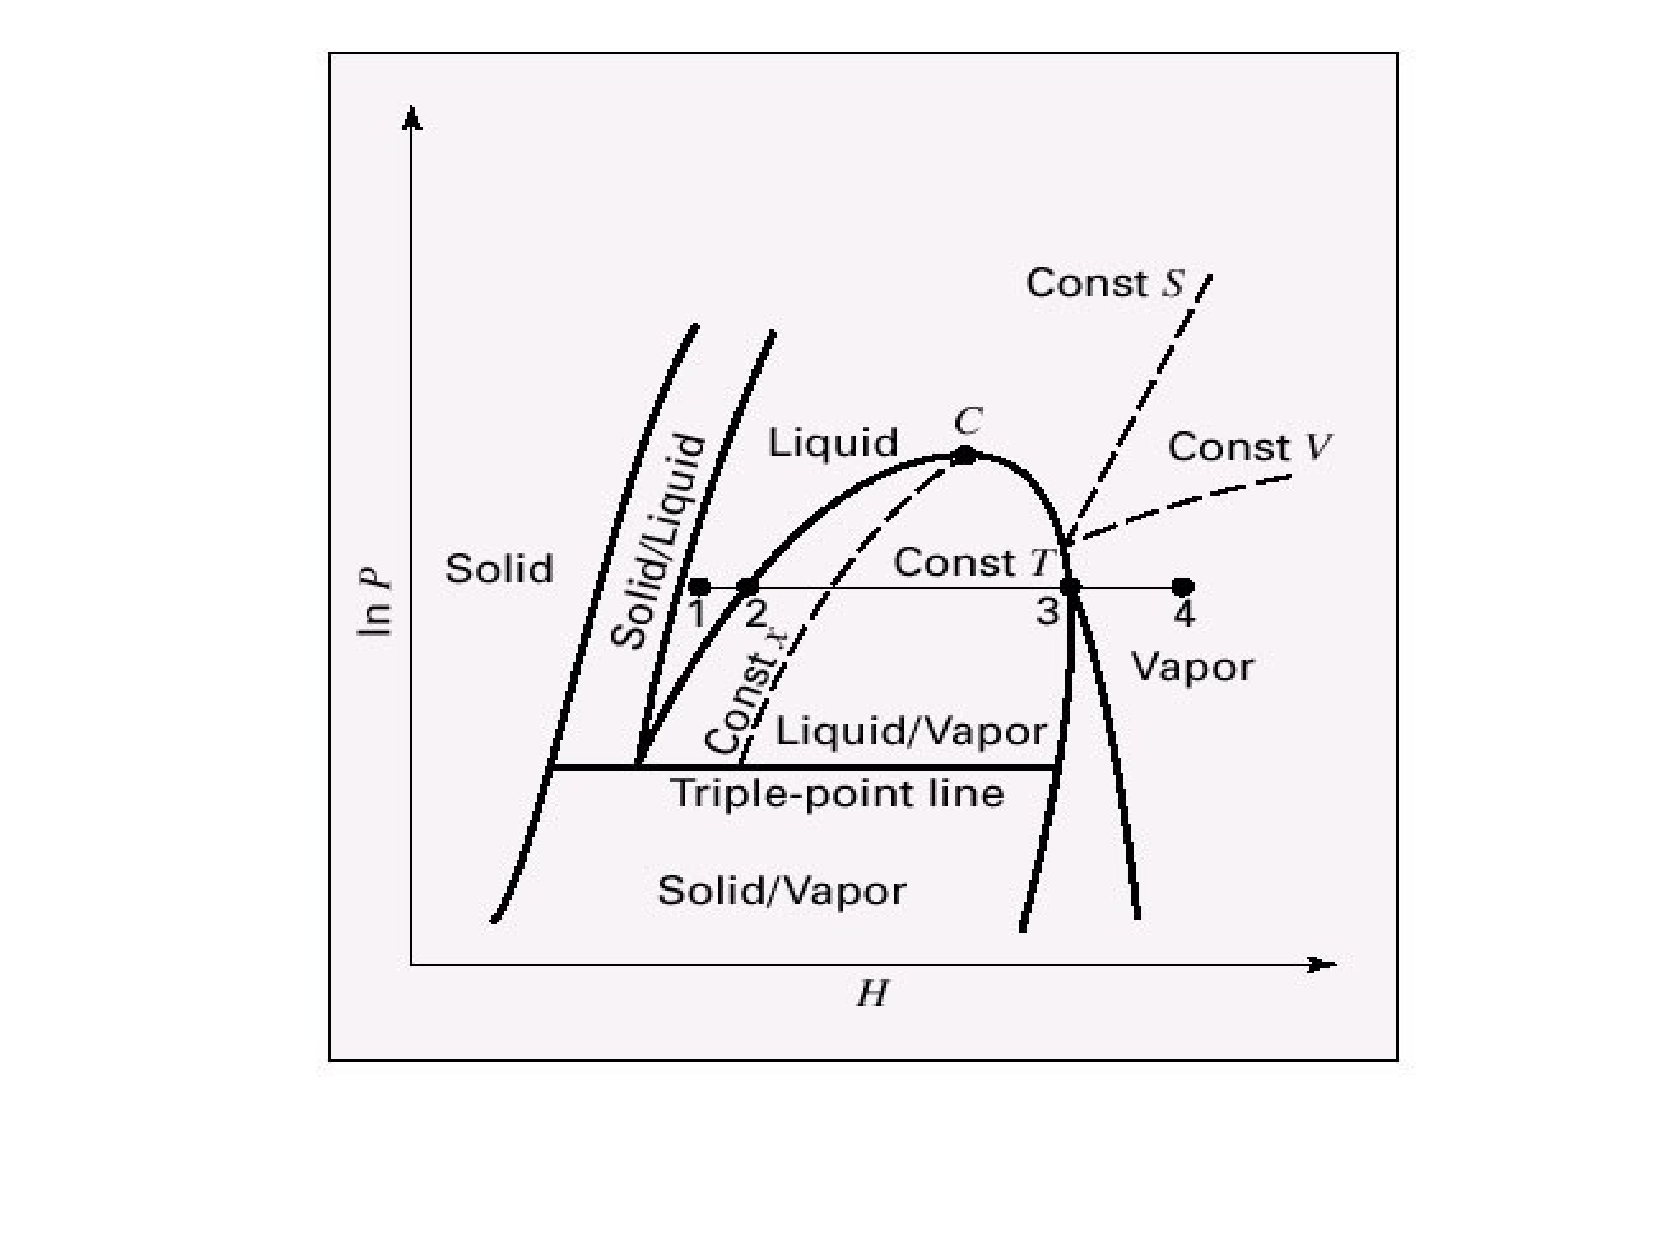
\includegraphics[width=1\columnwidth,clip]{./../Pics/LnP_H_Diagram}
        \end{center}
      \end{figure}
\end{frame}
\normalsize


%%%
%%% Slide
%%%
%\scriptsize
\begin{frame}
  \frametitle{Temperature $\times$ Entropy ({\it TS}) Diagram}
      \begin{figure}%
        \begin{center}
          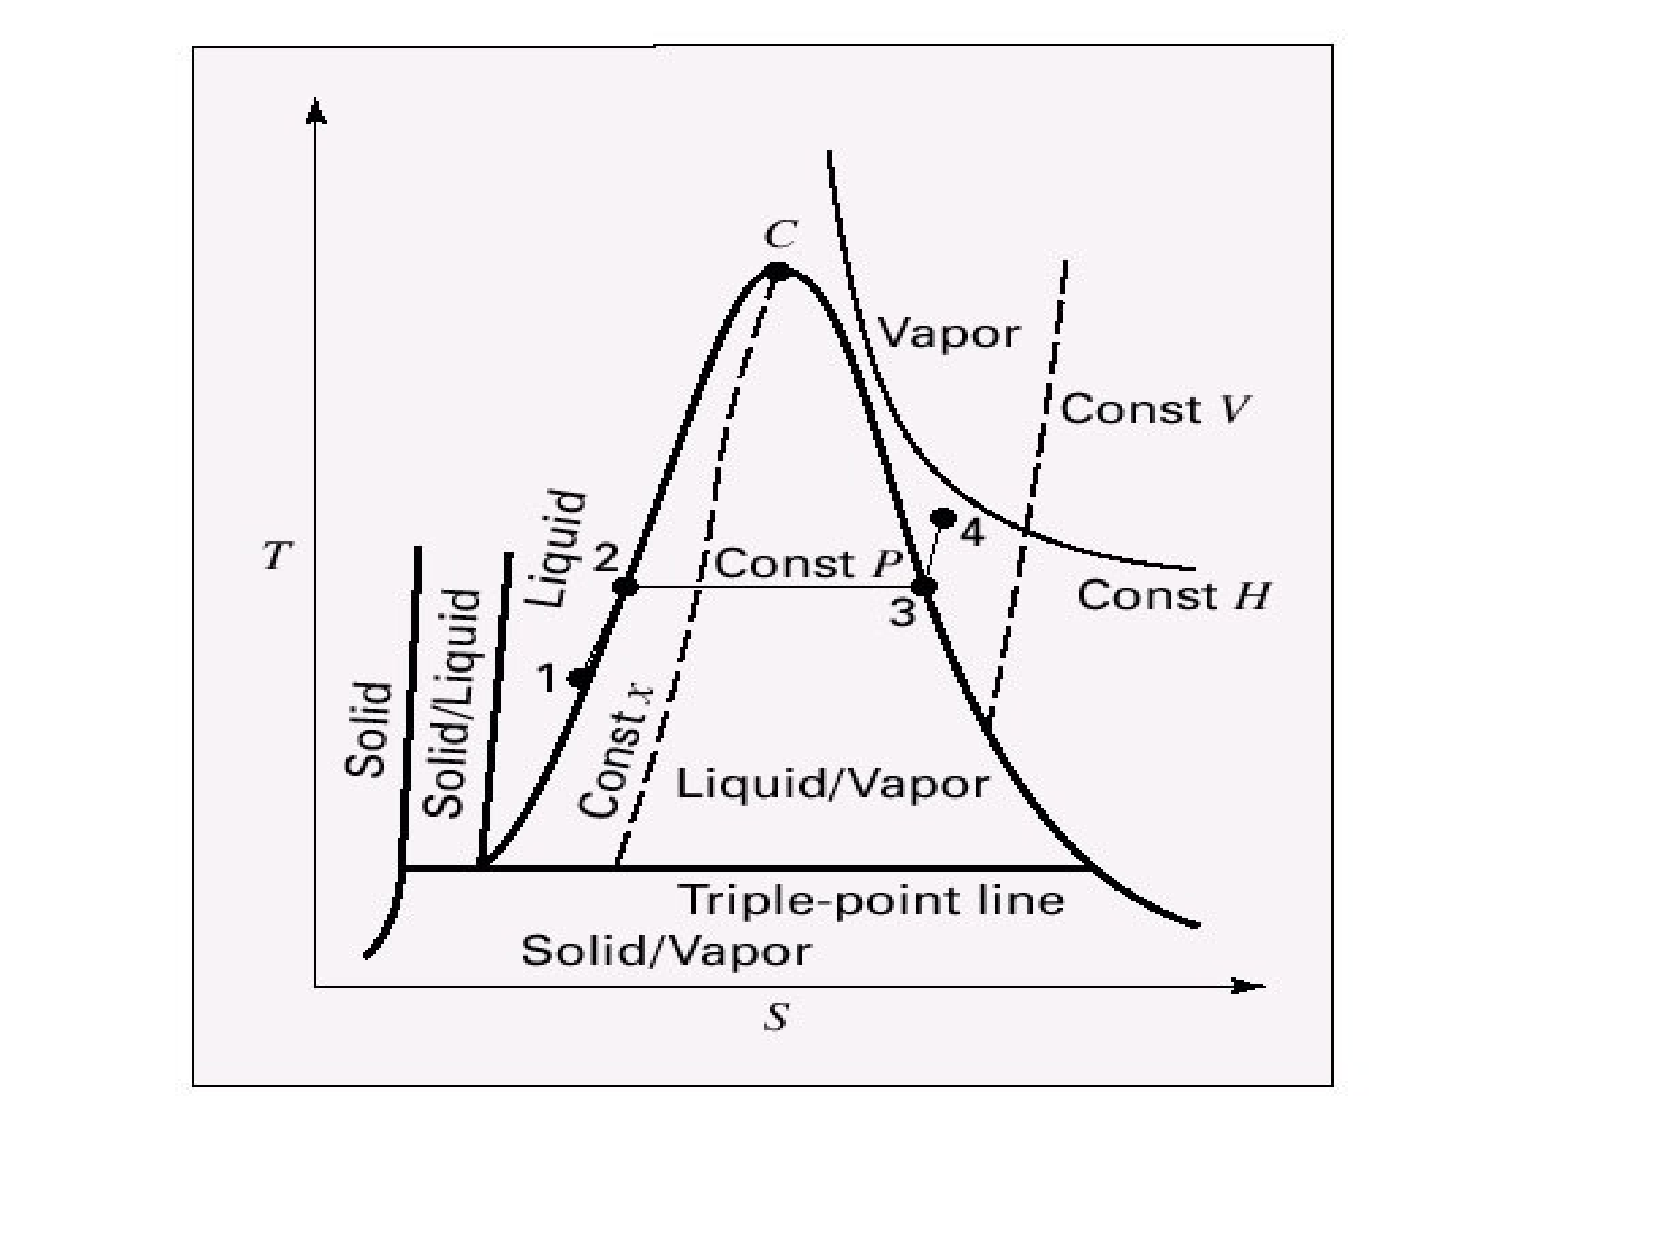
\includegraphics[width=1\columnwidth,clip]{./../Pics/T_S_Diagram}
        \end{center}
      \end{figure}
\end{frame}
\normalsize

%%%
%%% Slide
%%%
%\scriptsize
\begin{frame}
  \frametitle{Enthalpy $\times$ Entropy ({\it Moiller}) Diagram}
      \begin{figure}%
        \begin{center} 
          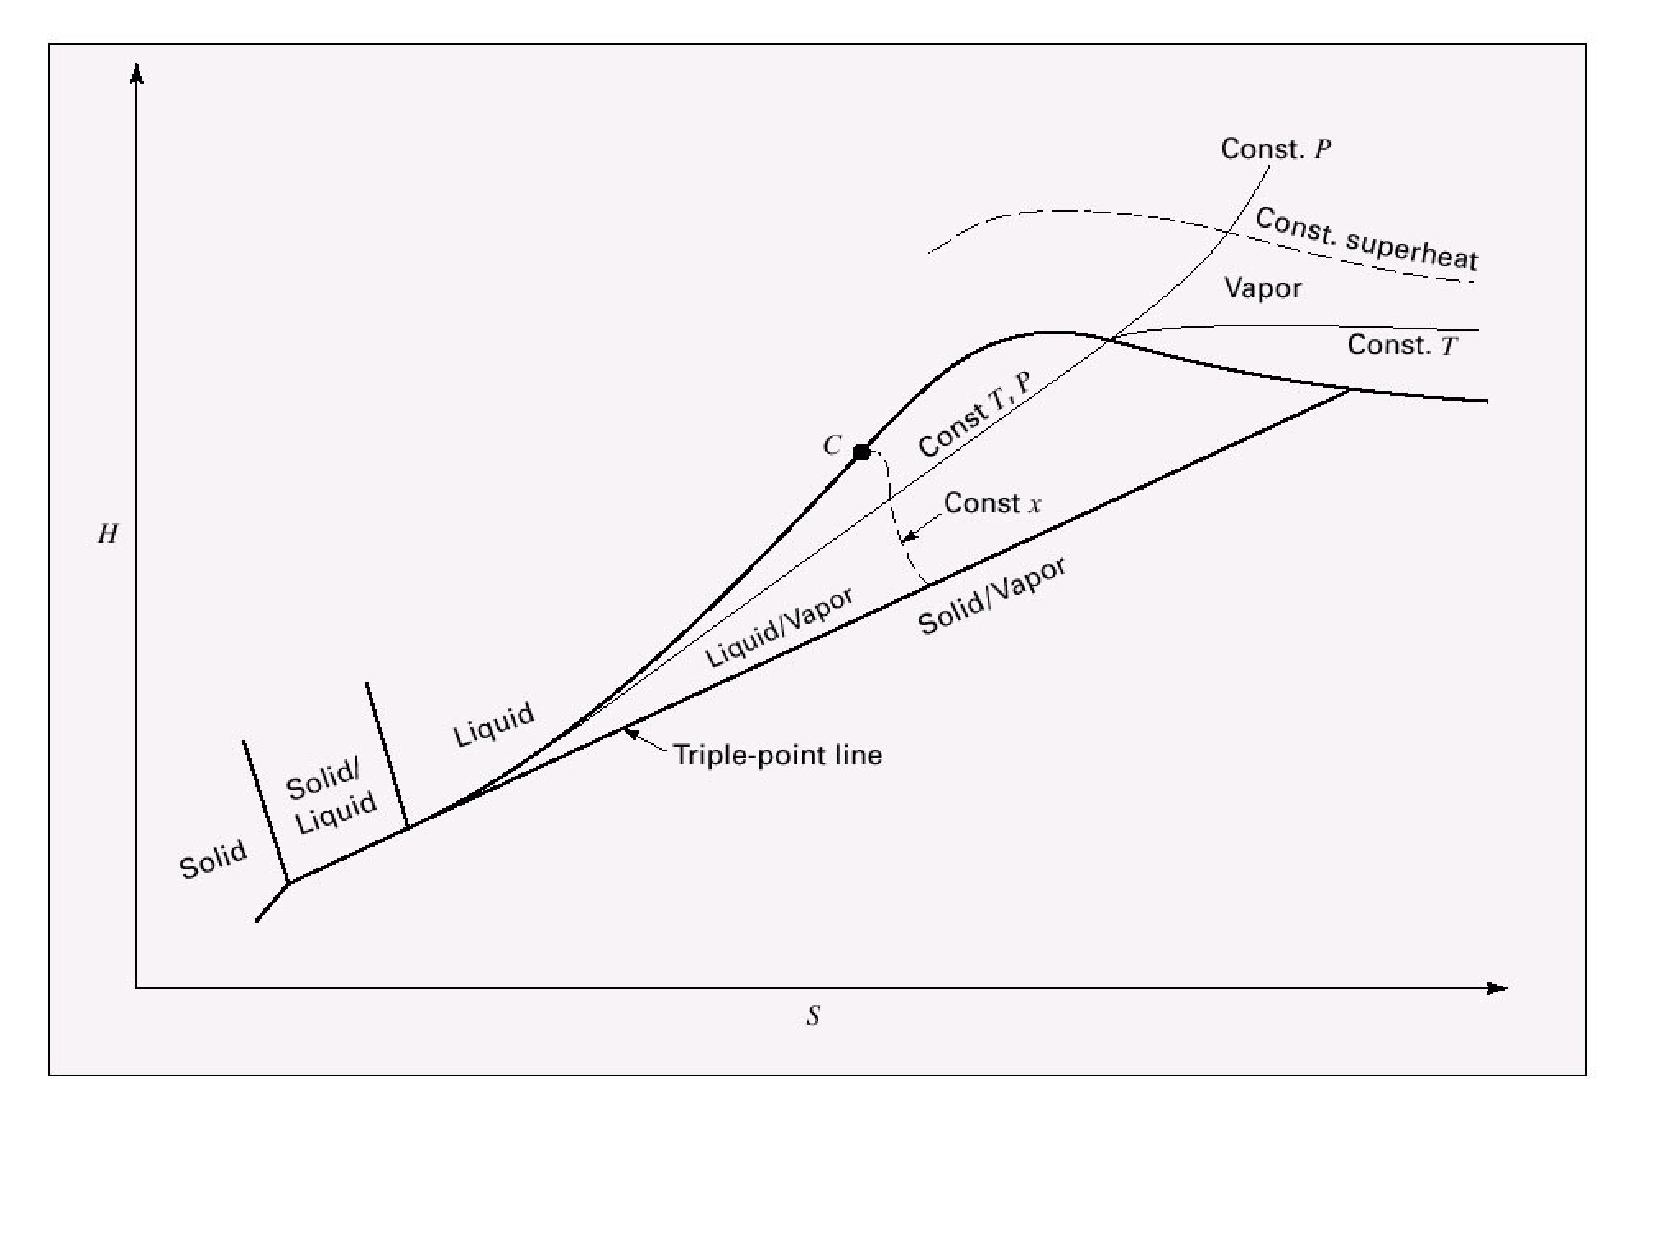
\includegraphics[width=1\columnwidth,clip]{./../Pics/MoillerDiagram}
        \end{center}
      \end{figure}
\end{frame}
\normalsize
\end{comment}
%%%
%%%  COMMENT
%%%

\section{Summary}

%%%
%%% Slide
%%%
%\scriptsize
\begin{frame}
 \frametitle{Summary}
   \begin{enumerate}[1.]
     \item New thermodynamic potential properties: Gibbs and Helmholtz free energies;
     \item Introduction of Maxwell's relations and applications;
     \item Internal energy, enthalpy, entropy Gibbs and Helmholtz energies described as functions of pressure, volume and temperature (PVT);
     \item Introduction of residual properties;
     \item Two-phase systems.
   \end{enumerate}
\end{frame}

\begin{comment}
\section{Examples}

%%%
%%% Slide
%%%
%\scriptsize
\begin{frame}
   \frametitle{Example 1}%[label=Module03:Example01]
    \blue{A block of copper of 1 kg undertakes a reversible compression from 0.1 MPa to 100 MPa at constant temperature of 15$^{\circ}$C. Calculate:}
    \begin{enumerate}[a)]
       \item \blue{Work done on the copper block during the process;}
       \item \blue{Change in entropy {\it per} kg of copper;}
       \item \blue{Heat transfer and;}
       \item \blue{Change of internal energy {\it per} kg.}
    \end{enumerate}
    \blue{Given, }
    \begin{itemize}
       \item \blue{Volume expansivity coefficient: $\beta = 5\times 10^{-5}$ K$^{-1}$;}
       \item \blue{Isothermal compressibility coefficient: $\kappa = 8.6\times 10^{-12}$ m$^{2}$.N$^{-1}$;}
       \item \blue{specific volume: $v=1.14\times 10^{-4}$ m$^{3}$.kg$^{-1}$.}
    \end{itemize} 

    \noindent{\bf Solution:} 

    \visible<2->{{\bf(a)} The work done during the compression,
                \begin{displaymath}
                   w = -\int P dv,
                \end{displaymath}
                where $v$ is the specific volume.}\visible<3->{ $\kappa$ was defined in Module 2 as,
                \begin{displaymath}
                   \kappa = \frc{1}{v}\left(\frc{\partial v}{\partial P}\right)_{T}\;\Longrightarrow \; v\kappa dP = - dv \;\;\text{ (with constant T)}
                \end{displaymath}}
                For isothermal processes
                \begin{displaymath}
                   w = -\int P dv = - \int P\left(-v\kappa dP\right) = \frc{v}{2}\kappa\left(P_{2}^{2}-P_{1}^{2}\right) = 4.90 \frc{\text{J}}{\text{kg}}
                \end{displaymath}

\end{frame}

%%%
%%% Slide
%%%
%\scriptsize
\begin{frame}
   \frametitle{Example 1}

    \visible<1->{For isothermal processes
                \begin{displaymath}
                   w = -\int P dv = - \int P\left(-v\kappa dP\right) = \frc{v}{2}\kappa\left(P_{2}^{2}-P_{1}^{2}\right) = 4.90 \frc{\text{J}}{\text{kg}}
                \end{displaymath}}
    
   \visible<2->{{\bf (b)} $ds$ = ? (specific entropy).}

   \visible<3->{From the Maxwell relations, 
                \begin{displaymath}
                   -\left(\frc{\partial s}{\partial P}\right)_{T} = \left(\frc{\partial v}{\partial T}\right)_{P},
                \end{displaymath}} 

   \visible<4->{and from the definition of $\beta$,
                \begin{eqnarray}
                    && \beta = \frc{1}{v}\left(\frc{\partial v}{\partial T}\right)_{P} \;\;\Longrightarrow\;\; -\left(\frc{\partial s}{\partial P}\right)_{T} = \beta v \nonumber \\
                    && ds = -\beta v dP \;\;\Longrightarrow ds = s_{2}-s_{1} = -\beta v \left(P_{2}-P_{1}\right) = -0.5694 \frc{\text{J}}{\text{kg.K}} \nonumber
                \end{eqnarray}}

\end{frame}

%%%
%%% Slide
%%%
%\scriptsize
\begin{frame}
   \frametitle{Example 1}

    \visible<1->{{\bf (c)} The heat transferred in such reversible isothermal process is
                \begin{displaymath}
                   dq = Tds \;\;\Longrightarrow q = T\left(s_{2}-s_{1}\right) = -164.07 \frc{\text{J}}{\text{kg}}.
                \end{displaymath}}

    \visible<1->{{\bf (d)} The specific internal energy,
                \begin{eqnarray}
                   &&  du = q + w \nonumber \\
                   && \left(u_{2}-u_{1}\right) = \underbrace{-164.07}_{\text{heat removed from the system}} + \overbrace{4.90}^{\text{work given to the system}} = -159.17 \frc{\text{J}}{\text{kg}}. \nonumber
                \end{eqnarray}}

\end{frame}



%%%
%%% Slide
%%%
%\scriptsize
\begin{frame}
   \frametitle{Example 2}
    \blue{Demonstrate that the derivative of molar volume \wrt temperature at constant pressure is}
     \begin{displaymath}
         \blue{\Partial[V]{T}{P} = -\frc{\Partial[P]{T}{V}}{\Partial[P]{V}{T}},}
     \end{displaymath}
     \blue{and obtain an expression for $\Partial[V]{T}{P}$ for the van der Waals EOS.} \\

   \blue{ {\bf Hint:} You should start the proof from the total differential of a continuous function $f(a,b)$,}
     \begin{displaymath}
         \blue{df = \Partial[f]{a}{b}da + \Partial[f]{b}{a}db.}
     \end{displaymath}

\end{frame}


%%%
%%% Slide
%%%
%\scriptsize
\begin{frame}
   \frametitle{Example 2}

    \noindent{\bf Solution:} 
    \visible<1->{The total differential of a generic continuous function $f(a,b)$ is
       \begin{displaymath}
           df = \Partial[f]{a}{b}da + \Partial[f]{b}{a}db.
       \end{displaymath}
       where (from the given thermodynamic function) $f=P$, $a=T$ and $b=V$, \ie}

    \visible<2->{\begin{displaymath}
          dP = \Partial[P]{T}{V}dT + \Partial[P]{V}{T}dV.
       \end{displaymath}}

    \visible<3->{However we want a differential expression in which $P$ is constant, therefore} \visible<4->{$\mathbf{dP = 0}$,}
       \begin{eqnarray}
           \visible<5->{0 &=& \Partial[P]{T}{V}dT + \Partial[P]{V}{T}dV \;\;\;\text{ at } P \text{ constant},}\nonumber \\
           \visible<6->{\Partial[V]{T}{P} &=& -\frc{\Partial[P]{T}{V}}{\Partial[P]{V}{T}}.} \nonumber
       \end{eqnarray}

\end{frame}

%%%
%%% Slide
%%%
%\scriptsize
\begin{frame}
   \frametitle{Example 2}

    \visible<1->{Now we want to obtain a differential expression for the vdW-EOS,}
    \visible<2->{\begin{displaymath}
          P = \frc{RT}{V-b} - \frc{a}{V^{2}},
       \end{displaymath}
       where $V$ is the molar volume and $a$ and $b$ are constants that {\it depends only on critical properties}, $P_{c}$ and $T_{c}$.} 

    \visible<3->{Due to the non-linearity of this EOS, obtaining $\Partial[V]{T}{P}$ from a direct differentiation would be difficult. However, now we know an expression that cn help us,}

    \visible<4->{\begin{displaymath}
         \Partial[V]{T}{P} = -\frc{\Partial[P]{T}{V}}{\Partial[P]{V}{T}} = -\frc{\frc{R}{V-b}}{-\frc{RT}{\left(V-b\right)^{2}+\frc{2a}{V^{3}}}}
     \end{displaymath} }

\end{frame}


%%%
%%% Slide
%%%
%\scriptsize
\begin{frame}
   \frametitle{Example 3}
    \blue{Derive an expression for enthalpy change of a gas during an isothermal process assuming using the following EOS: $P\left(V-b\right)=RT$}

    \noindent\visible<2->{{\bf Solution:} We have seen that enthalpy change is given by (see Slide 8 or Eqn. 36a from the {\it Notes})
    \begin{displaymath}
       dH = C_{p}dT + \left[V - T\Partial[V]{T}{P}\right]dP.
    \end{displaymath}}

    \visible<3->{We can rearrange the EOS and obtain $\Partial[V]{T}{P}$, (or, for a more complex EOS, we could use the procedure of Exmaple 2 to obtain this differential)}
    \begin{eqnarray}
       \visible<3->{&& P\left(V-b\right)=RT \;\;\;\rightarrow\;\;\; V = \frc{RT}{P} + b \;\;\;\rightarrow\;\;\; \Partial[V]{T}{P} = \frc{R}{P}\;\;\text{ thus, }} \nonumber \\
       \visible<3->{&& dH = C_{p}dT + \left(V - \frc{RT}{P}\right)dP = \blue{C_{p}dT + bdP}.} \nonumber 
    \end{eqnarray}

\end{frame}

%%%
%%% Slide
%%%
%\scriptsize
\begin{frame}
   \frametitle{Example 4}
    \blue{The Antoine equation constants for toluene are $A=14.01415$, $B=3106.46$ K and $C=-53.15$ K (for pressure given in kPa). At 1.01325$\times$10$^{5}$ Pa, calculate:}
        \begin{enumerate}[(a)]
           \item \blue{the boiling temperature and;}
           \item \blue{the enthalpy of vaporisation at these conditions.}
        \end{enumerate}

    \noindent\visible<2->{{\bf Solution:} }
       \begin{enumerate}[a)]
%
           \item<2->Boiling temperature can be calculated from the Antoine equation,
               \begin{eqnarray}
                   \visible<3->{&& \ln{P^{\text{sat}}} = A - \frc{B}{T+C}} \nonumber \\
                   \visible<4->{&& T = \frc{B}{A-\ln{P^{\text{sat}}}} - C = \blue{383.77 \text{ K}}}  \nonumber          
               \end{eqnarray}
%
           \item<5-> The enthalpy of vaporisation, $\Delta H^{\text{fg}}$, can be obtained from the Clausius-Clapeyron equation,
               \begin{eqnarray}
                   && \visible<5->{\frc{d}{dT} \left(\ln{P^{\text{sat}}}\right) = \frc{\Delta H^{\text{fg}}}{RT^{2}}} \nonumber \\
                   && \visible<6->{\frc{B}{\left(T+C\right)^{2}} =  \frc{\Delta H^{\text{fg}}}{RT^{2}} \;\;\Longrightarrow \Delta H^{\text{fg}} = \blue{34.7984 \text{ kJ.mol}^{-1}}.} \nonumber
               \end{eqnarray}
%
        \end{enumerate}

\end{frame}

%%%
%%% Slide
%%%
%\scriptsize
\begin{frame}
   \frametitle{Example 5}
    \blue{Steam (dry and saturated) is supplied by the boiler at 15 bar and the condenser inlet pressure is 0.4 bar. Calculate the Rankine efficiency of the cycle. Neglect the pump work, assume the enthalpy of fluid leaving the pump is 317.58 kJ.kg$^{-1}$.}
    \noindent\visible<2->{{\bf Solution:} For this problem, let's assume the same numbering of Fig. 7a in the Lecture-Notes.}\visible<3->{ At 15 bar, dry and saturated $\left(\ie\; x_{1}=1\right)$ steam} \visible<4->{has the following properties (from saturated table),}
           \visible<4->{\begin{eqnarray}
             T_{1} &=& T_{\text{sat}} = 198.3^{\circ}\text{C},\nonumber \\
             h_{1} &=& h_{\text{g}} = 2792.2\; \text{kJ.kg}^{-1} \nonumber \\
             s_{1} &=& s_{\text{g}} = 6.4448\; \text{kJ.(kg.K)}^{-1} \nonumber
          \end{eqnarray} }
          \visible<5->{In the condenser, $P_{2}=0.4$ bar,
          \begin{eqnarray}
              T_{2} &=& T_{\text{sat}} = 75.87^{\circ}\text{C}, \nonumber \\
              h_{\text{g}2} &=& 2636.8\;\text{kJ.kg}^{-1},\;\;\; h_{\text{f}2} = 317.58\;\text{kJ.kg}^{-1},  \nonumber \\
              s_{\text{g}2} &=& 7.6700 \;\text{kJ.(kg.K)}^{-1},\;\;\; s_{\text{f}2} = 1.0259\;\text{kJ.(kg.K)}^{-1}. \nonumber  
          \end{eqnarray}}
\end{frame}

%%%
%%% Slide
%%%
%\scriptsize
\begin{frame}
   \frametitle{Example 5}
         \visible<1-> {$h_{2}$ and $s_{2}$ depend on the knowledge of how vaporised the water is, in other words, we need to determine the quality of the steam, $x_{1}$ through},
         \begin{displaymath}
              \visible<2->{M = \mfr[M]{}{L} + \mfr[x]{}{V}\Delta\mfr[M]{}{LV}}
              \visible<3->{ \begin{cases}
                      h_{2} = h_{\text{f}2} + x_{2}\left(h_{\text{g}2} - h_{\text{f}2}\right), \\
                      s_{2} = s_{\text{f}2} + x_{2}\left(s_{\text{g}2} - s_{\text{f}2}\right).  
              \end{cases}}
         \end{displaymath}

         \visible<4-> {As we know that water is expanded isentropically in the turbine, \ie \blue{$s_{1}=s_{2}$},}
         \begin{eqnarray}
             && \visible<5-> {s_{2} = s_{\text{f}2} + x_{2}\left(s_{\text{g}2} - s_{\text{f}2}\right) = s_{1} = 6.4448}  \nonumber \\
             && \visible<6-> {x_{2} = 0.8156 \;\;(81.56\% \text{ of vapour})}\nonumber
         \end{eqnarray}

         \visible<7-> {Thus replacing in 
             \begin{displaymath}
                h_{2} = h_{\text{f}2} + x_{2}\left(h_{\text{g}2} - h_{\text{f}2}\right) = 2209.14\text{ kJ.kg}^{-1}.
             \end{displaymath}}

         \visible<8-> {The Rankine efficiency is given by}
             \begin{displaymath}
                 \visible<8-> {\eta_{\text{Rankine}} = \frc{\text{Adiabatic or Isentropic Heat Drop}}{\text{Heat Supplied}} =} \visible<9-> {\frc{\left|h_{1}-h_{2}\right|}{h_{1}-h_{\text{f}4}} = 0.2356\;\;\;\rightarrow \;\;\; 23.56\%}
             \end{displaymath}
\end{frame}

\end{comment} 

\end{document}
 
